\chapter{Marco teórico}
\label{Chapter2}

Este capítulo del marco teórico tiene como objetivo presentar una visión general de la bibliografía relevante al
objetivo de la tesis. En la primera sección, se explorará la historia del reconocimiento de dígitos por parte de las
computadoras y las técnicas desarrolladas. Posteriormente, se brindará un breve resumen de la evolución de las redes
neuronales, con especial atención en las redes densas y convolucionales, y sus conceptos básicos. La sección siguiente
se enfocará en el aprendizaje por transferencia de las redes neuronales, sus capacidades y limitaciones. Finalmente, se
profundizará en la adaptación de dominio y se explicarán las distintas técnicas utilizadas en el trabajo.

\section{Reconocimiento de dígitos}

El reconocimiento de caracteres por parte de las computadoras ha sido un campo de investigación activo durante varias
décadas. Una de las primeras investigaciones en este campo se centró en cómo las neuronas del cerebro procesan y
reconocen información visual.

En \citeyear{hubel1959receptive}, \citeauthor{hubel1959receptive} comenzaron a investigar la percepción visual en el
cerebro de los gatos. Descubrieron que las neuronas en la corteza visual primaria del cerebro de los gatos respondían a
estímulos visuales específicos, como líneas y bordes. Además, identificaron dos tipos de células en la corteza visual
primaria: células simples y células complejas. Las células simples respondían a estímulos visuales específicos, como
barras de luz en una dirección particular, mientras que las células complejas respondían a estímulos visuales más
complejos, como patrones en movimiento. En 1981, recibieron el Premio Nobel de Fisiología o Medicina por su trabajo en
el procesamiento visual del cerebro.

Inspirado por el trabajo de \citeauthor{hubel1959receptive}, en 1980 se desarrolló la red Neocognitron \parencite{fukushima1980neocognitron}. La red Neocognitron fue uno de los primeros modelos de aprendizaje profundo
utilizados para el reconocimiento de caracteres. La red estaba compuesta por múltiples capas, cada una de las cuales
procesaba información visual en diferentes niveles de abstracción.

A pesar de que la red Neocognitron fue un gran avance en el reconocimiento de caracteres, todavía tenía limitaciones.
En particular, la red no podía reconocer caracteres escritos a mano que eran muy diferentes de los caracteres que se
habían utilizado para entrenar la red.

A fines de la década de 1980, se presentó un enfoque importante para el reconocimiento de dígitos escritos a mano
llamado ``Sistema Neuronal de Reconocimiento de Dígitos'' \parencite{lecun1989backpropagation}. Este sistema utilizó una red neuronal de varias capas y fue entrenado utilizando el
método de retropropagación del error. El modelo tuvo un rendimiento significativamente mejor que los enfoques
anteriores y sentó las bases para el desarrollo de sistemas de reconocimiento de dígitos escritos a mano más
sofisticados.

En la década de 1990, se desarrollaron otros modelos de aprendizaje profundo que superaron las limitaciones de los
enfoques anteriores. \cite{lecun1995learning} se menciona por primera vez el término de {\it red convolucional}.

Desde entonces, los algoritmos de reconocimiento de caracteres han seguido evolucionando y mejorando. Actualmente, los
sistemas de reconocimiento de caracteres son capaces de reconocer caracteres escritos a mano con una precisión cercana
al 100\%. Además del reconocimiento de caracteres, estas técnicas también se han utilizado para la detección de objetos
en imágenes y videos, así como para la traducción automática.

\section{Redes Neuronales}
\cite{mcculloch1943logical} estudiaron y propusieron un modelo del comportamiento de la
neurona biológica. La neurona artificial que propusieron fue un sistema binario que consiste en que si la suma de entradas excitatorias supera un umbral de activación, y además no
hay una entrada inhibitoria, la neurona se activa y emite una respuesta; en caso contrario, la neurona no se activa.

En \citeyear{hebb1949organization} se propone que estas redes podían aprender. Este hecho estaba relacionado con la
conductividad de la sinapsis. Así, la repetida activación de una neurona por otra, a través de una sinapsis
determinada, aumenta su conductividad y la hace más propensa a ser activada sucesivamente, induciendo a la formación de
un circuito de neuronas estrechamente conectadas entre sí \parencite{hebb1949organization}.

Años más tarde, \cite{rosenblatt1958perceptron} propone un modelo de neurona llamadas perceptrones basadas en el modelo
de McCulloch-Pitts. El mayor logro de Rosenblatt fue que pudo demostrar que, flexibilizando algunas de las reglas de la
McCulloch-Pitts (la inhibición absoluta, la contribución igual de todas las entradas, etc), las neuronas artificiales
podían aprender de los datos. Y lo que es más importante, ideó un algoritmo de aprendizaje supervisado para este modelo
de neurona que permitía averiguar los pesos correctos directamente a partir de los datos de entrenamiento. La sencillez
y eficacia de este algoritmo de aprendizaje para problemas linealmente separables son algunas de las razones clave por
las que se hizo tan popular a finales de los años cincuenta y principios de los sesenta. Sin embargo, esta popularidad
hizo que Rosenblatt exagerara la capacidad de aprendizaje de su perceptrón, dando lugar a expectativas poco realistas
en la comunidad científica y/o también difundidas por los medios de comunicación.

En \citeyear{minsky1969perceptrons}, se publica un libro en el cual se expone la naturaleza lineal de los perceptrones
y de sus limitadas capacidades \parencite{minsky1969perceptrons}. A raíz de este evento es que se inicia el denominado ``invierno de la inteligencia
artificial'' de los 1980s, donde cesó el interés de la comunidad por los modelos conexionistas.

La contribución más importante en la reemergencia del conexionismo en los años ochenta fue la técnica {\it
backpropagation} desarrollada por \cite{rumelhart1986learning}. En realidad, esta técnica fue desarrollada inicialmente
por \cite{werbos1974beyond} y después redescubierta por varios grupos de investigadores \parencite{lecun1985learning, rumelhart1986learning}. Este algoritmo abrió las puertas al uso práctico de las redes
neuronales en un sinfín de campos. La idea detrás del {\it backpropagation} es ajustar los pesos de una red neuronal
para minimizar el error de predicción en un conjunto de datos de entrenamiento. Este error se calcula como la
diferencia entre la salida real de la red y la salida deseada para una entrada dada. Para ajustar los pesos de la red,
se utilizan las derivadas parciales del error con respecto a cada uno de los pesos, lo que permite actualizar los pesos
en la dirección que minimiza el error. El entrenamiento de una red utilizando {\it backpropagation} se divide en dos
fases: la propagación hacia adelante y la propagación hacia atrás. En la fase de propagación hacia adelante, se calcula
la salida de la red para una entrada dada. La salida de la red se compara con la salida deseada para calcular el error
de predicción. En la fase de propagación hacia atrás, se utiliza este error para calcular las derivadas parciales del
error con respecto a cada uno de los pesos de la red. Este algoritmo ajusta los pesos en la dirección que minimiza el
error de la red, multiplicando la derivada parcial del error por una tasa de aprendizaje y restando el resultado del
peso correspondiente.

Las redes neuronales más ``simples'' entrenadas con {\it backpropagation}, son las denominadas redes multicapa
alimentadas hacia delante ({\it feed forward}) o perceptrones mutlicapa {\it MLP}. En
\citeyear{funahashi1989approximate}, se demuestra teóricamente que una red de este tipo, con una capa oculta y el
suficiente número de nodos, puede aproximar cualquier función continua con cualquier grado de precisión \parencite{funahashi1989approximate}.

\subsection{Redes Densas}
Como se detalló anteriormente, los perceptrones son modelos lineales incapaces de resolver problemas que no sean
linealmente separables por un hiperplano. Una forma de solventar esta situación es encadenar un conjunto de
perceptrones para crear redes neuronales densas (ver figura \ref{fig:nn}). La predicción $\hat{y}$ de una red es una
generalización directa de la predicción de un perceptrón. Primero se calculan las activaciones $a_i^1$ de los nodos de
la capa oculta $h_i^1$ en función de las entradas $x_i$ y los pesos de entrada $w_i^1$. Luego, se calculan las
activaciones $a_i^2$ de la unidad de salida $h_1^2$ dadas las activaciones de la capa anterior y los pesos $w_i^2$.

\begin{figure}[H]
  \centering

  \tikzset{every picture/.style={line width=0.75pt}} %set default line width to 0.75pt        

  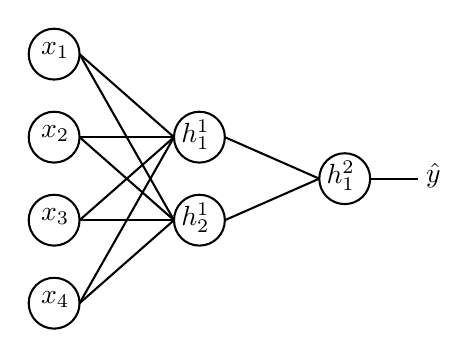
\begin{tikzpicture}[x=0.75pt,y=0.75pt,yscale=-1,xscale=1]
    %uncomment if require: \path (0,300); %set diagram left start at 0, and has height of 300

    %Shape: Circle [id:dp4714623984365989] 
    \draw   (0,12.25) .. controls (0,5.48) and (5.48,0) .. (12.25,0) .. controls (19.02,0) and (24.5,5.48) .. (24.5,12.25) .. controls (24.5,19.02) and (19.02,24.5) .. (12.25,24.5) .. controls (5.48,24.5) and (0,19.02) .. (0,12.25) -- cycle ;

    %Shape: Circle [id:dp25434586654127544] 
    \draw   (0,52.25) .. controls (0,45.48) and (5.48,40) .. (12.25,40) .. controls (19.02,40) and (24.5,45.48) .. (24.5,52.25) .. controls (24.5,59.02) and (19.02,64.5) .. (12.25,64.5) .. controls (5.48,64.5) and (0,59.02) .. (0,52.25) -- cycle ;

    %Shape: Circle [id:dp9726011815419306] 
    \draw   (0,92.25) .. controls (0,85.48) and (5.48,80) .. (12.25,80) .. controls (19.02,80) and (24.5,85.48) .. (24.5,92.25) .. controls (24.5,99.02) and (19.02,104.5) .. (12.25,104.5) .. controls (5.48,104.5) and (0,99.02) .. (0,92.25) -- cycle ;

    %Shape: Circle [id:dp2291699685520565] 
    \draw   (0,132.25) .. controls (0,125.48) and (5.48,120) .. (12.25,120) .. controls (19.02,120) and (24.5,125.48) .. (24.5,132.25) .. controls (24.5,139.02) and (19.02,144.5) .. (12.25,144.5) .. controls (5.48,144.5) and (0,139.02) .. (0,132.25) -- cycle ;

    %Shape: Circle [id:dp14614955000159813] 
    \draw   (70,52.25) .. controls (70,45.48) and (75.48,40) .. (82.25,40) .. controls (89.02,40) and (94.5,45.48) .. (94.5,52.25) .. controls (94.5,59.02) and (89.02,64.5) .. (82.25,64.5) .. controls (75.48,64.5) and (70,59.02) .. (70,52.25) -- cycle ;

    %Shape: Circle [id:dp8388103519245029] 
    \draw   (70,92.25) .. controls (70,85.48) and (75.48,80) .. (82.25,80) .. controls (89.02,80) and (94.5,85.48) .. (94.5,92.25) .. controls (94.5,99.02) and (89.02,104.5) .. (82.25,104.5) .. controls (75.48,104.5) and (70,99.02) .. (70,92.25) -- cycle ;

    %Shape: Circle [id:dp7556907650297429] 
    \draw   (140,72.25) .. controls (140,65.48) and (145.48,60) .. (152.25,60) .. controls (159.02,60) and (164.5,65.48) .. (164.5,72.25) .. controls (164.5,79.02) and (159.02,84.5) .. (152.25,84.5) .. controls (145.48,84.5) and (140,79.02) .. (140,72.25) -- cycle ;

    %Straight Lines [id:da8929189573178169] 
    \draw    (24.5,12.25) -- (70,52.25) ;
    %Straight Lines [id:da5905797689118961] 
    \draw    (24.5,52.25) -- (70,52.25) ;
    %Straight Lines [id:da8059054934899097] 
    \draw    (24.5,92.25) -- (70,52.25) ;
    %Straight Lines [id:da18480058250239084] 
    \draw    (24.5,132.25) -- (70,52.25) ;
    %Straight Lines [id:da9649216528295181] 
    \draw    (24.5,12.25) -- (70,92.25) ;
    %Straight Lines [id:da2593081377394073] 
    \draw    (24.5,52.25) -- (70,92.25) ;
    %Straight Lines [id:da23945860731626256] 
    \draw    (24.5,92.25) -- (70,92.25) ;
    %Straight Lines [id:da45284543126132815] 
    \draw    (24.5,132.25) -- (70,92.25) ;
    %Straight Lines [id:da8439890580329283] 
    \draw    (94.5,52.25) -- (140,72.25) ;
    %Straight Lines [id:da026411209066727226] 
    \draw    (94.5,92.25) -- (140,72.25) ;
    %Straight Lines [id:da46511217961352624] 
    \draw    (164.5,72.25) -- (187.75,72.25) ;

    % Text Node
    \draw (4.5,5) node [anchor=north west][inner sep=0.75pt]    {$x_{1}$};
    % Text Node
    \draw (4.5,45) node [anchor=north west][inner sep=0.75pt]    {$x_{2}$};
    % Text Node
    \draw (4.5,85) node [anchor=north west][inner sep=0.75pt]    {$x_{3}$};
    % Text Node
    \draw (4.5,125) node [anchor=north west][inner sep=0.75pt]    {$x_{4}$};
    % Text Node
    \draw (72,42.4) node [anchor=north west][inner sep=0.75pt]    {$h_{1}^{1}$};
    % Text Node
    \draw (72,82.4) node [anchor=north west][inner sep=0.75pt]    {$h_{2}^{1}$};
    % Text Node
    \draw (142,62.4) node [anchor=north west][inner sep=0.75pt]    {$h_{1}^{2}$};
    % Text Node
    \draw (190,63.4) node [anchor=north west][inner sep=0.75pt]    {$\hat{y}$};

  \end{tikzpicture}
  \caption[Red neuronal densa]{Red neuronal con una capa de entrada de 4 características, una capa oculta de 2 neuronas y una capa de salida con 1 neurona.}
  \label{fig:nn}
\end{figure}

La única diferencia entre este cálculo y el del perceptrón es que las unidades ocultas calculan una función no lineal
de sus entradas. Generalmente es llamada como {\it función de activación} o {\it función de enlace}. Formalmente, si
$w_{i,d}$ son los pesos que conectan las entradas $d$ a la unidad oculta $i$, entonces la activación de la unidad $i$
se calcula como:

\begin{align}
  h_i = f(\mathbf{w}_i \cdot \mathbf{x} + b_i)
\end{align}

Donde $f$ es la función de activación, $\mathbf{w}_i$ es el vector de pesos que alimentan el nodo $i$ y $b_i$ es el
término de {\it bias}. Existen múltiples funciones de activación, las más comunes son:

\begin{itemize}
  \item Tangente hiperbólica: $f(x) = tanh(x) = \frac{e^x - e^{-x}}{e^x + e^{-x}}$
  \item Función sigmoidea: $f(x) = \sigma(x) = \frac{1}{1+exp(-x)}$
  \item ReLU: $f(x) = max(0, x)$
  \item Softmax: $f(x_i) = \sigma(x_i) = \frac{e^{x_{i}}}{\sum_{j=1}^K e^{x_{j}}} \ \ \ para\ i=1,2,\dots,K$
\end{itemize}

\subsection{Redes Convolucionales}
Una de las principales limitaciones de las redes densas es su incapacidad para manejar datos que presentan una
estructura espacial, como imágenes o audio. Esta limitación se debe principalmente al problema de la invarianza
espacial, donde una misma entidad (por ejemplo, el dígito '6') puede tener diferentes ubicaciones en una imagen. Dado
que las redes densas tratan cada entrada de manera aislada, ignorando las relaciones espaciales entre ellas, es posible
que no detecten patrones o características importantes en los datos, lo que puede reducir su rendimiento.

Para solucionar este problema, surgió la idea de utilizar redes neuronales convolucionales (CNN). Estas redes se basan
en utilizar capas de neuronas que comparten pesos y realizan una operación de convolución en los datos de entrada. Esto
permite que la red tenga una mayor capacidad para detectar patrones y características en los datos, ya que las neuronas
de las capas de convolución están compartiendo información y pueden detectar patrones a diferentes escalas y en
diferentes posiciones de los datos.

Matemáticamente, la operación de convolución se puede representar como:

\begin{equation}
  (f * g)(x) = \int_{-\infty}^{\infty} f(t)g(x-t) dt
  \label{eq:convolucion}
\end{equation}

Donde $f$ y $g$ son dos funciones y $*$ es el operador de convolución. Esta operación consiste en desplazar la función
$g$ a través de la función $f$ y multiplicar cada valor de $f$ por el valor de $g$ en esa posición. El resultado de la
operación de convolución es una nueva función que refleja la combinación de los valores de $f$ y $g$.

En la figura \ref{fig:convolucion-ejemplo} se ilustra el proceso de cálculo de una convolución para escenarios
discretos. Para una matriz $I$ de tamaño $6\times6$ y un filtro $K$ de tamaño $3\times3$, la operación de convolución
$*$ en una CNN aplica el filtro $K$ deslizándolo sobre la matriz $I$ para producir $I*K$.

\begin{figure}[H]
  \centering
  \convoutionpicture 42
  \caption[Operador {\it convolución}]{Ejemplo de una convolución para una matriz $I$ y un filtro o kernel $K$, produciendo la matriz $I*K$.}
  \label{fig:convolucion-ejemplo}
\end{figure}

En una CNN, la matriz $I$ representa la imagen y el filtro $K$ es el conjunto de parámetros entrenables del modelo,
análogo a las neuronas en una red densa. Aunque existen filtros estudiados para detectar ciertas características, como
el filtro Sobel para detectar bordes, se permite que la red aprenda de forma autónoma $K$ con el fin de detectar las
características relevantes $I*K$ para la tarea a través del entrenamiento. Esto permite que la red encuentre
características sin el sesgo que se introduciría al utilizar únicamente filtros predefinidos.

Una de las principales ventajas de las CNNs es que son capaces de procesar datos con una gran cantidad de dimensiones,
como imágenes con altura, anchura y profundidad (canales de color). Esto se debe a que las capas de convolución son
capaces de realizar operaciones de filtrado sobre los datos de entrada, permitiendo a la red aprender características
específicas de los datos de manera eficiente. Además, las CNNs tienen la capacidad de generalizar de manera efectiva,
lo que significa que son capaces de realizar buenas predicciones en conjuntos de datos desconocidos.

Otra ventaja de las CNN es que cuentan con capas de {\it pooling} o también llamadas de submuestreo. Su objetivo
principal es reducir el tamaño espacial de la representación de características para disminuir la cantidad de
parámetros y de operaciones necesarias en la red, lo que permite reducir el costo computacional y evitar el
sobreajuste. Además, al reducir el tamaño de la representación, se logra una cierta invarianza en las características
aprendidas por la red, lo que significa que la posición exacta de las características dentro de la imagen ya no importa
tanto. La operación de {\it pooling} en una CNN consiste en dividir la imagen de entrada en subregiones no superpuestas
y aplicar una función a cada subregión. En general, existen tres tipos de funciones que se utilizan en {\it pooling}:
{\it max pooling}, que toma el valor máximo de cada subregión; {\it average pooling}, que toma el valor promedio de
cada subregión; y {\it min pooling}, que toma el valor mínimo de cada subregión. La figura \ref{fig:maxpool-ejemplo}
ilustra el cálculo de {\it max pooling} a la matriz $I*K$ del ejemplo anterior.

\begin{figure}[H]
  \centering

  \begin{tikzpicture}
    % ------- style -------
    \tikzset{%
      parenthesized/.style={%
          left delimiter  = (,
          right delimiter = ),
        },
      node distance = 10mu,
    }

    \matrix[matrix of math nodes, parenthesized, ampersand replacement=\&] (I*K) {
      1 \& 5 \& 2 \& 3 \\
      3 \& 2 \& 4 \& 2 \\
      1 \& 4 \& 2 \& 1 \\
      3 \& 2 \& 1 \& 1 \\
    };

    \node (arrow) [right = of I*K] {${} \xRightarrow{\text{maxpool}}  {}$};

    \matrix[matrix of math nodes, parenthesized, ampersand replacement=\&] (maxpool) [right = of arrow] {
      5 \& 4 \\
      4 \& 2 \\
    };

    % ------- highlighting -------
    \newcommand{\padding}{0pt}

    \def\rowResult{1}
    \def\colResult{1}
    \begin{scope}[on background layer]
      \coordinate (Is-nw) at ([xshift=-\padding, yshift=+\padding] I*K-\rowResult-\colResult.north west);
      \coordinate (Is-se) at ([xshift=+\padding, yshift=-\padding] I*K-\the\numexpr\rowResult+2-1\relax-\the\numexpr\colResult+2-1\relax.south east);

      \filldraw[red, fill opacity=.1] (Is-nw) rectangle (Is-se);
      \filldraw[red, fill opacity=.1] (maxpool-\rowResult-\colResult.north west) rectangle (maxpool-\rowResult-\colResult.south east);
    \end{scope}

    \def\rowResult{1}
    \def\colResult{2}
    \begin{scope}[on background layer]
      \coordinate (Is-nw) at ([xshift=-\padding, yshift=+\padding] I*K-\rowResult-\the\numexpr\colResult+1\relax.north west);
      \coordinate (Is-se) at ([xshift=+\padding, yshift=-\padding] I*K-\the\numexpr\rowResult+1\relax-\the\numexpr\colResult+2\relax.south east);

      \filldraw[green, fill opacity=.1] (Is-nw) rectangle (Is-se);
      \filldraw[green, fill opacity=.1] (maxpool-\rowResult-\colResult.north west) rectangle (maxpool-\rowResult-\colResult.south east);
    \end{scope}

    \def\rowResult{2}
    \def\colResult{1}
    \begin{scope}[on background layer]
      \coordinate (Is-nw) at ([xshift=-\padding, yshift=+\padding] I*K-\the\numexpr\rowResult+1\relax-\the\numexpr\colResult+0\relax.north west);
      \coordinate (Is-se) at ([xshift=+\padding, yshift=-\padding] I*K-\the\numexpr\rowResult+2\relax-\the\numexpr\colResult+1\relax.south east);

      \filldraw[blue, fill opacity=.1] (Is-nw) rectangle (Is-se);
      \filldraw[blue, fill opacity=.1] (maxpool-\rowResult-\colResult.north west) rectangle (maxpool-\rowResult-\colResult.south east);
    \end{scope}

    \def\rowResult{2}
    \def\colResult{2}
    \begin{scope}[on background layer]
      \coordinate (Is-nw) at ([xshift=-\padding, yshift=+\padding] I*K-\the\numexpr\rowResult+1\relax-\the\numexpr\colResult+1\relax.north west);
      \coordinate (Is-se) at ([xshift=+\padding, yshift=-\padding] I*K-\the\numexpr\rowResult+2\relax-\the\numexpr\colResult+2\relax.south east);

      \filldraw[yellow, fill opacity=.1] (Is-nw) rectangle (Is-se);
      \filldraw[yellow, fill opacity=.1] (maxpool-\rowResult-\colResult.north west) rectangle (maxpool-\rowResult-\colResult.south east);
    \end{scope}

    % ------- labels -------
    \tikzset{node distance=0em}
    \node[below=of I*K] (I*K-label) {$I*K$};
    \node at (maxpool |- I*K-label) {$maxpool(I*K)$};

  \end{tikzpicture}

  \caption[Operador {\it maxpool}]{Maxpool $2\times2$ aplicado al ejemplo de la figura \ref{fig:convolucion-ejemplo} $I*K$.}
  \label{fig:maxpool-ejemplo}
\end{figure}

Las redes neuronales convolucionales tienen una gran variedad de aplicaciones prácticas en diferentes campos, algunas
de las cuales incluyen:
\begin{itemize}
  \item Reconocimiento de imágenes: CNN se utilizan ampliamente en tareas de clasificación de imágenes, como el reconocimiento
        de objetos, el análisis de sentimientos en imágenes, la generación de descripciones automáticas para imágenes, entre
        otras \parencite{krizhevsky2017imagenet}.
  \item Análisis de videos: CNN también se utilizan en tareas de análisis de videos, como el seguimiento de objetos, la
        detección de eventos, la generación de subtítulos automáticos para videos, entre otras \parencite{simonyan2014twostream}.
  \item Procesamiento de lenguaje natural: CNN también se utilizan en tareas de procesamiento de lenguaje natural, como la
        clasificación de texto, la generación de texto, el análisis de sentimientos y la traducción automática \parencite{bugnon2020dl4papers}.
  \item Medicina: CNN se utilizan en tareas de diagnóstico médico, como la detección de cáncer de mama, la detección de
        enfermedades cardíacas, la detección de problemas en imágenes médicas, entre otras \parencite{wang2016deep}.
\end{itemize}

\subsection{Arquitecturas}

Existen distintos tipos de arquitecturas de redes neuronales convolucionales debido a que cada una tiene diferentes
fortalezas y debilidades en términos de capacidad de generalización, extracción de características y rendimiento \parencite{lecun2015deep}. Algunos factores que pueden influir en la elección de una arquitectura en particular incluyen \parencite{he2016deep}:

\begin{itemize}
  \item Tamaño de los datos de entrada: para procesar grandes conjuntos de datos, es posible que se necesite una red con una
        mayor capacidad de procesamiento y una mayor cantidad de parámetros.
  \item Nivel de detalle de las características: algunas arquitecturas pueden ser más eficientes para detectar características
        a diferentes escalas y en diferentes posiciones, mientras que otras pueden tener una mayor capacidad para detectar
        patrones complejos.
  \item Nivel de generalización: algunas arquitecturas pueden ser más capaces de generalizar a datos nuevos y menos vistos
        durante el entrenamiento, mientras que otras pueden ser más propensas a sobreajuste.
  \item Requerimientos de tiempo y recursos: algunas arquitecturas pueden requerir más tiempo y recursos para entrenar y
        evaluar, lo que puede ser un factor importante a considerar dependiendo de los objetivos del proyecto.
\end{itemize}

Una arquitectura simple de CNN para la clasificación de imágenes es la ilustrada en la figura \ref{fig:cnn}: una subred
convolucional $\mathcal{G}$ que extrae información y genera características $\mathbf{f}$ a partir de la entrada
$\mathbf{x}$; y una subred densa $\mathcal{C}$ que se encarga de clasificar las características aprendidas $\mathbf{f}$
en las etiquetas del problema $\mathbf{\hat{y}}$.

\begin{figure}[H]
  \centering

  \tikzset{every picture/.style={line width=0.75pt}} %set default line width to 0.75pt        

  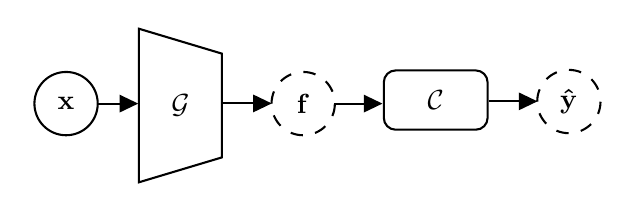
\begin{tikzpicture}[x=0.75pt,y=0.75pt,yscale=-1,xscale=1]
    %uncomment if require: \path (0,300); %set diagram left start at 0, and has height of 300

    %Shape: Circle [id:dp5607633409516137] 
    \draw   (40.33,108.25) .. controls (40.33,99.83) and (47.16,93) .. (55.58,93) .. controls (64.01,93) and (70.83,99.83) .. (70.83,108.25) .. controls (70.83,116.67) and (64.01,123.5) .. (55.58,123.5) .. controls (47.16,123.5) and (40.33,116.67) .. (40.33,108.25) -- cycle ;
    %Shape: Trapezoid [id:dp8058596397440787] 
    \draw   (90.67,72.17) -- (130.67,84.17) -- (130.67,134.17) -- (90.67,146.17) -- cycle ;
    %Straight Lines [id:da42639122448642897] 
    \draw    (70.83,108.25) -- (87.33,108.25) ;
    \draw [shift={(90.33,108.25)}, rotate = 180] [fill={rgb, 255:red, 0; green, 0; blue, 0 }  ][line width=0.08]  [draw opacity=0] (8.93,-4.29) -- (0,0) -- (8.93,4.29) -- cycle    ;
    %Shape: Circle [id:dp6831404033749999] 
    \draw  [dash pattern={on 4.5pt off 4.5pt}] (154.58,108.25) .. controls (154.58,99.83) and (161.41,93) .. (169.83,93) .. controls (178.26,93) and (185.08,99.83) .. (185.08,108.25) .. controls (185.08,116.67) and (178.26,123.5) .. (169.83,123.5) .. controls (161.41,123.5) and (154.58,116.67) .. (154.58,108.25) -- cycle ;
    %Rounded Rect [id:dp3958441794745311] 
    \draw   (208.67,97.98) .. controls (208.67,94.82) and (211.23,92.26) .. (214.38,92.26) -- (252.95,92.26) .. controls (256.11,92.26) and (258.67,94.82) .. (258.67,97.98) -- (258.67,115.12) .. controls (258.67,118.27) and (256.11,120.83) .. (252.95,120.83) -- (214.38,120.83) .. controls (211.23,120.83) and (208.67,118.27) .. (208.67,115.12) -- cycle ;
    %Straight Lines [id:da33421369991474537] 
    \draw    (131.33,108.17) -- (151.67,108.17) ;
    \draw [shift={(154.67,108.17)}, rotate = 180] [fill={rgb, 255:red, 0; green, 0; blue, 0 }  ][line width=0.08]  [draw opacity=0] (8.93,-4.29) -- (0,0) -- (8.93,4.29) -- cycle    ;
    %Straight Lines [id:da30712807219538707] 
    \draw    (184.67,108.25) -- (205,108.25) ;
    \draw [shift={(208,108.25)}, rotate = 180] [fill={rgb, 255:red, 0; green, 0; blue, 0 }  ][line width=0.08]  [draw opacity=0] (8.93,-4.29) -- (0,0) -- (8.93,4.29) -- cycle    ;
    %Shape: Circle [id:dp6313033137153481] 
    \draw  [dash pattern={on 4.5pt off 4.5pt}] (282.58,107.25) .. controls (282.58,98.83) and (289.41,92) .. (297.83,92) .. controls (306.26,92) and (313.08,98.83) .. (313.08,107.25) .. controls (313.08,115.67) and (306.26,122.5) .. (297.83,122.5) .. controls (289.41,122.5) and (282.58,115.67) .. (282.58,107.25) -- cycle ;
    %Straight Lines [id:da8576886251233382] 
    \draw    (259.33,107.17) -- (279.67,107.17) ;
    \draw [shift={(282.67,107.17)}, rotate = 180] [fill={rgb, 255:red, 0; green, 0; blue, 0 }  ][line width=0.08]  [draw opacity=0] (8.93,-4.29) -- (0,0) -- (8.93,4.29) -- cycle    ;

    \draw (110.67,109.17) node   [align=left] {\begin{minipage}[lt]{22.78pt}\setlength\topsep{0pt}
        \begin{center}
          $\mathcal{G}$
        \end{center}

      \end{minipage}};
    \draw (233.67,106.73) node   [align=left] {\begin{minipage}[lt]{26.23pt}\setlength\topsep{0pt}
        \begin{center}
          $\mathcal{C}$
        \end{center}

      \end{minipage}};
    \draw (169.83,108.25) node   [align=left] {\begin{minipage}[lt]{21.08pt}\setlength\topsep{0pt}
        \begin{center}
          $\mathbf{f}$
        \end{center}

      \end{minipage}};
    \draw (297.83,107.25) node   [align=left] {\begin{minipage}[lt]{21.08pt}\setlength\topsep{0pt}
        \begin{center}
          $\mathbf{\hat{y}}$
        \end{center}

      \end{minipage}};
    \draw (55.58,108.25) node   [align=left] {\begin{minipage}[lt]{21.08pt}\setlength\topsep{0pt}
        \begin{center}
          $\mathbf{x}$
        \end{center}

      \end{minipage}};

  \end{tikzpicture}

  \caption[Red neuronal convolucional]{Arquitectura de una red convolucional simple. Las entradas $\mathbf{x}$ son procesadas por una red convolucional $\mathcal{G}$
    que generan características $\mathbf{f}$ para luego ser clasificadas por una red densa $\mathcal{C}$ en $\mathbf{\hat{y}}$.}
  \label{fig:cnn}
\end{figure}

Tal es el caso de la red LeNet, que fue propuesta por \cite{lecun1998gradient}. Esta red consta de dos capas de
convolución seguidas por dos capas densas y una capa de salida, y fue utilizada con éxito para el reconocimiento de
números escritos a mano en el conjunto de datos MNIST.

Por otro lado, una arquitectura de red neuronal convolucional más compleja es la red ResNet (abreviación de Residual
Network), propuesta por \cite{he2016deep}. Estas redes están diseñadas para resolver el problema de la propagación del
gradiente en las redes neuronales profundas, lo que permite entrenar modelos con una gran cantidad de capas.

\subsubsection{LeNet}
LeNet es una de las primeras arquitecturas de redes neuronales de aprendizaje profundo desarrolladas para tareas de
reconocimiento de caracteres escritos a mano. Aunque la arquitectura original de LeNet es bastante antigua, su diseño
sigue siendo relevante hoy en día y se utiliza como una arquitectura básica para tareas similares.

\begin{figure}[H]
  \centering
  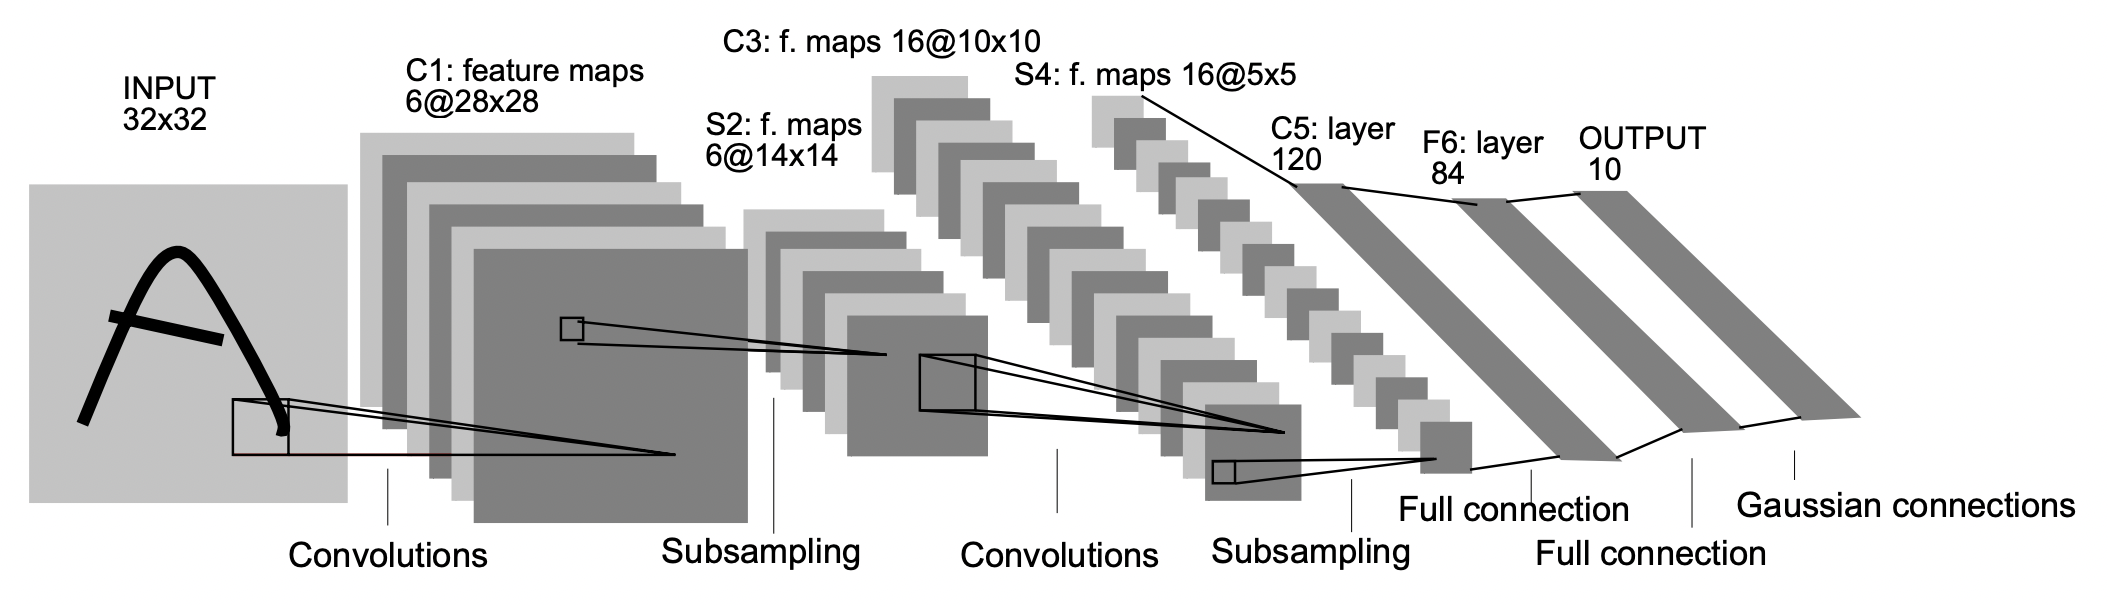
\includegraphics[width=0.9\textwidth]{chapter2/lenet5.png}

  \caption[Arquitectura de una LeNet-5]{Arquitectura de una LeNet-5. Imagen tomada de \cite{lecun1998gradient}.}
  \label{fig:lenet}
\end{figure}

El desarrollo de la LeNet implicó la aparición de las CNNs y sus componentes básicos. No obstante, no fue popular en su
momento debido a la falta del hardware necesario para entrenarlas y otros algoritmos como las máquinas de vectores de
soporte (SVM por sus siglas en inglés) que podían obtener resultados similares o superadores \parencite{lecun1998gradient, decoste2002training, lauer2007trainable}.

En 2012, Alex Krizhevsky ganó la competencia de ImageNet con su arquitectura AlexNet \parencite{krizhevsky2017imagenet}, basada en la LeNet pero con modificaciones. La principal diferencia entre ambas es la
complejidad y profundidad de la arquitectura, con AlexNet teniendo ocho capas y más de 60 millones de parámetros
entrenables, mientras que LeNet tiene cinco capas y menos de un millón de parámetros. Además, AlexNet utiliza filtros
convolucionales más grandes (11x11 y 5x5) que permiten capturar características de imagen más grandes y complejas, y
técnicas de regularización más avanzadas, como el dropout, para prevenir el sobreajuste. En contraste, LeNet utiliza
filtros más pequeños (5x5 y 3x3) y técnicas de regularización más simples como la regularización L2.

Desde el éxito de AlexNet, las CNNs se han convertido en la mejor opción para aplicaciones de visión computacional y se
han creado muchos tipos diferentes de CNN, como las redes R-CNN utilizada para detección y segmentación de objetos \parencite{girshick2014rich}. En la actualidad los modelos CNN son bastante diferentes de LeNet, pero todos se desarrollan
sobre la base de LeNet.

\subsubsection{ResNet}

La idea principal detrás de las redes ResNet es la utilización de {\it bloques residuales} en lugar de las capas
tradicionales de la red neuronal. Un bloque residual se compone de varias capas de una red neuronal tradicional, pero
con una conexión residual que permite que la información de entrada se sume directamente a la salida de las capas
internas. Esto permite que la información se propague de manera más eficiente a través de las capas profundas de la
red, lo que ayuda a reducir el problema del desvanecimiento de gradientes en la retropropagación del error.

Además, las redes ResNet también utilizan una técnica llamada {\it bottleneck} que reduce el número de canales de
salida en las capas internas del bloque residual, lo que ayuda a reducir el número de parámetros y mejorar la
eficiencia del modelo obligando a la red a aprender características más relevantes.

Las redes neuronales ResNet se han desarrollado en diferentes arquitecturas, cada una de las cuales tiene su propio
conjunto de características y aplicaciones. Las mismas son:

\begin{itemize}
  \item ResNet18 y ResNet34 \parencite{he2016deep}: son arquitecturas de ResNet con un número moderado de capas (18 y 34 respectivamente) que se
        utilizan comúnmente en tareas de clasificación de imágenes y reconocimiento de objetos.
  \item ResNet50, ResNet101 y ResNet152 \parencite{he2016deep}: son arquitecturas de ResNet con un mayor número de capas (50, 101 y 152 respectivamente) que se
        utilizan comúnmente en tareas de detección de objetos y segmentación de imágenes. Estas arquitecturas tienen una mayor
        capacidad representativa y son más precisas en las tareas de aprendizaje profundo complejas, pero requieren más tiempo
        de entrenamiento y recursos.
  \item ResNet-S y ResNet-M \parencite{sandler2018mobilenetv2}: son arquitecturas de ResNet que se utilizan en dispositivos móviles y sistemas de baja
        potencia. Estas arquitecturas son más ligeras en términos de parámetros y requisitos de cálculo que las arquitecturas
        anteriores.
  \item ResNeXt \parencite{xie2017aggregated}: es una variante de ResNet que utiliza una técnica llamada {\it agrupación cardinal} para
        mejorar la capacidad representativa de la red. Esta técnica utiliza varios grupos de canales en lugar de uno solo para
        mejorar la capacidad representativa del modelo y lograr mejores resultados en tareas de clasificación y reconocimiento.
\end{itemize}

\section{Aprendizaje por transferencia}

El aprendizaje por transferencia es una técnica que consiste en utilizar lo que se ha aprendido en una tarea para
mejorar el rendimiento en otra tarea relacionada \parencite{thrun1998learning}. Esta técnica se aplica comúnmente en el contexto de redes neuronales, especialmente en
tareas de imágenes, y se basa en la idea de que algunos conocimientos adquiridos en una tarea pueden ser reutilizados
en otra tarea, lo que permite que la red aprenda de manera más eficiente y con menos datos. Ha ganado popularidad en
los últimos años debido a la creciente cantidad de datos disponibles y a la necesidad de entrenar modelos más complejos
y de mayor rendimiento.

En el contexto de las redes neuronales, el aprendizaje por transferencia se puede llevar a cabo de varias maneras, como
el {\it pre-entrenamiento} y el {\it fine-tuning}. El pre-entrenamiento es una técnica de aprendizaje por transferencia
en la que se entrena una red en una tarea y luego se utiliza como punto de partida para entrenar otra red en una tarea
diferente \parencite{erhan2010does}. Esto permite que la red aprenda de manera más rápida y con menos datos, ya que ya ha adquirido
algunos conocimientos en la primera tarea. El pre-entrenamiento se puede llevar a cabo de varias maneras, como por
ejemplo entrenando una red en un conjunto de datos de gran tamaño y luego utilizándola como inicialización para una
tarea específica de menor tamaño. Esto se ha utilizado con éxito en varias tareas de aprendizaje automático, como la
clasificación de imágenes \parencite{chen2021pretrained} y el procesamiento del lenguaje natural \parencite{liu2019text}. También se ha utilizado con éxito en el contexto de redes neuronales profundas, donde ha
demostrado ser una técnica efectiva para mejorar el rendimiento y la capacidad de generalización de las redes \parencite{girshick2014rich}.

Por otro lado, el fine-tuning es una técnica en la que se utilizan las capas de una red pre-entrenada en una tarea como
capas fijas en otra red que se entrena en una tarea diferente \parencite{yosinski2014transferable}. Esto permite que la red aprenda de manera más rápida y con menos datos \parencite{howard2018universal}.

\section{Adaptación de Dominio}
El {\it pre-entrenamiento} y el {\it fine-tuning} han mejorado considerablemente el estado del arte para diversos
problemas y aplicaciones del machine learning, incluso las redes profundas pre-entrenadas pueden adaptarse fácilmente a
tareas donde se cuenta con una pequeña cantidad de datos etiquetados. Sin embargo, en muchos escenarios prácticos, no
hay datos de entrenamiento etiquetados y, por lo tanto, existe la necesidad de transferir el aprendizaje de una red
profunda desde un dominio de origen en el que se dispone de datos de entrenamiento etiquetados a un dominio de destino
en el que solo existen datos sin etiquetar \parencite{glorot2011domain}. En esta situación, los modelos profundos siguen sufriendo degradaciones de rendimiento debido
al cambio de distribución \parencite{quinonero2008dataset}. Por lo tanto, se propone la {\it adaptación de dominio} para reducir el cambio de
distribución entre los dominios de entrenamiento y de prueba \parencite{jiang2022machine}.

Se han propuesto muchos métodos para la adaptación de dominios, ya sea ponderando o seleccionando muestras del dominio
de origen \parencite{sugiyama2007direct} o buscando una transformación de la distribución de origen a la distribución de destino \parencite{gong2013connecting}. Esta tesis analizará algunos de los métodos más comunes del ultimo caso.

\subsection{Domain Adversarial Neural Network}
Un gran hito al momento de modelar distribuciones es la Red Generativa Adversaria {\it GAN} \parencite{goodfellow2020generative}. Inspirada en estas arquitecturas GAN, la Red Neural Adversaria de Dominio {\it DANN} \parencite{ganin2016domain} consta de dos redes en la adaptación del dominio (figura \ref{fig:dann-esquema}). La primera es
la discriminadora de dominios $\mathcal{D}$ entrenada para distinguir las características de origen de las de destino y
la segunda es una generadora de características $\mathcal{G}$ que se entrena para confundir a $\mathcal{D}$ y
simultáneamente ayudar a la red clasificadora $\mathcal{C}$. La idea general es que $\mathcal{G}$ aprenda a generar
características lo suficientemente similares para ambos dominios de forma que $\mathcal{D}$ se equivoque y
$\mathcal{C}$ los clasifique correctamente.

\begin{figure}[H]
  \centering

  \tikzset{every picture/.style={line width=0.75pt}} %set default line width to 0.75pt        

  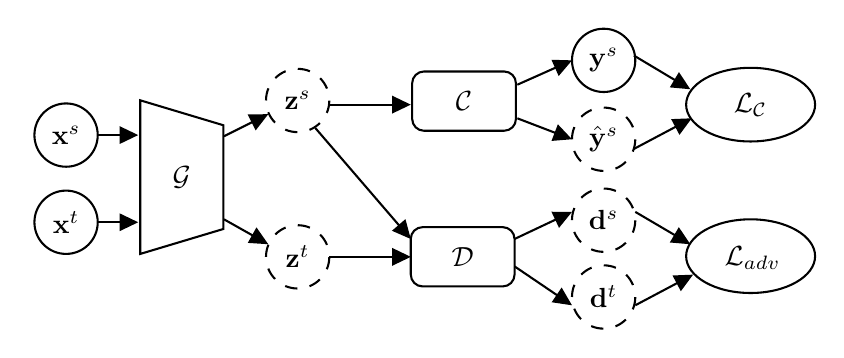
\begin{tikzpicture}[x=0.75pt,y=0.75pt,yscale=-1,xscale=1]
    \draw   (39,64.75) .. controls (39,56.33) and (45.83,49.5) .. (54.25,49.5) .. controls (62.67,49.5) and (69.5,56.33) .. (69.5,64.75) .. controls (69.5,73.17) and (62.67,80) .. (54.25,80) .. controls (45.83,80) and (39,73.17) .. (39,64.75) -- cycle ;

    \draw   (39,106.75) .. controls (39,98.33) and (45.83,91.5) .. (54.25,91.5) .. controls (62.67,91.5) and (69.5,98.33) .. (69.5,106.75) .. controls (69.5,115.17) and (62.67,122) .. (54.25,122) .. controls (45.83,122) and (39,115.17) .. (39,106.75) -- cycle ;

    \draw   (90,48) -- (130,60) -- (130,110) -- (90,122) -- cycle ;

    \draw    (69.5,64.75) -- (86,64.75) ;
    \draw [shift={(89,64.75)}, rotate = 180] [fill={rgb, 255:red, 0; green, 0; blue, 0 }  ][line width=0.08]  [draw opacity=0] (8.93,-4.29) -- (0,0) -- (8.93,4.29) -- cycle    ;
    \draw  [dash pattern={on 4.5pt off 4.5pt}] (150.58,48.08) .. controls (150.58,39.66) and (157.41,32.83) .. (165.83,32.83) .. controls (174.26,32.83) and (181.08,39.66) .. (181.08,48.08) .. controls (181.08,56.51) and (174.26,63.33) .. (165.83,63.33) .. controls (157.41,63.33) and (150.58,56.51) .. (150.58,48.08) -- cycle ;

    \draw  [dash pattern={on 4.5pt off 4.5pt}] (150.58,123.42) .. controls (150.58,114.99) and (157.41,108.17) .. (165.83,108.17) .. controls (174.26,108.17) and (181.08,114.99) .. (181.08,123.42) .. controls (181.08,131.84) and (174.26,138.67) .. (165.83,138.67) .. controls (157.41,138.67) and (150.58,131.84) .. (150.58,123.42) -- cycle ;

    \draw   (221,39.81) .. controls (221,36.65) and (223.56,34.1) .. (226.71,34.1) -- (265.29,34.1) .. controls (268.44,34.1) and (271,36.65) .. (271,39.81) -- (271,56.95) .. controls (271,60.11) and (268.44,62.67) .. (265.29,62.67) -- (226.71,62.67) .. controls (223.56,62.67) and (221,60.11) .. (221,56.95) -- cycle ;

    \draw   (220.33,114.81) .. controls (220.33,111.65) and (222.89,109.1) .. (226.05,109.1) -- (264.62,109.1) .. controls (267.77,109.1) and (270.33,111.65) .. (270.33,114.81) -- (270.33,131.95) .. controls (270.33,135.11) and (267.77,137.67) .. (264.62,137.67) -- (226.05,137.67) .. controls (222.89,137.67) and (220.33,135.11) .. (220.33,131.95) -- cycle ;

    \draw  [dash pattern={on 4.5pt off 4.5pt}] (298,105.75) .. controls (298,97.33) and (304.83,90.5) .. (313.25,90.5) .. controls (321.67,90.5) and (328.5,97.33) .. (328.5,105.75) .. controls (328.5,114.17) and (321.67,121) .. (313.25,121) .. controls (304.83,121) and (298,114.17) .. (298,105.75) -- cycle ;

    \draw  [dash pattern={on 4.5pt off 4.5pt}] (298,142.75) .. controls (298,134.33) and (304.83,127.5) .. (313.25,127.5) .. controls (321.67,127.5) and (328.5,134.33) .. (328.5,142.75) .. controls (328.5,151.17) and (321.67,158) .. (313.25,158) .. controls (304.83,158) and (298,151.17) .. (298,142.75) -- cycle ;

    \draw   (353,123.08) .. controls (353,113.28) and (366.91,105.33) .. (384.06,105.33) .. controls (401.22,105.33) and (415.13,113.28) .. (415.13,123.08) .. controls (415.13,132.89) and (401.22,140.83) .. (384.06,140.83) .. controls (366.91,140.83) and (353,132.89) .. (353,123.08) -- cycle ;

    \draw   (298,28.75) .. controls (298,20.33) and (304.83,13.5) .. (313.25,13.5) .. controls (321.67,13.5) and (328.5,20.33) .. (328.5,28.75) .. controls (328.5,37.17) and (321.67,44) .. (313.25,44) .. controls (304.83,44) and (298,37.17) .. (298,28.75) -- cycle ;
    \draw  [dash pattern={on 4.5pt off 4.5pt}] (298,66.75) .. controls (298,58.33) and (304.83,51.5) .. (313.25,51.5) .. controls (321.67,51.5) and (328.5,58.33) .. (328.5,66.75) .. controls (328.5,75.17) and (321.67,82) .. (313.25,82) .. controls (304.83,82) and (298,75.17) .. (298,66.75) -- cycle ;
    \draw   (353,50.08) .. controls (353,40.28) and (366.91,32.33) .. (384.06,32.33) .. controls (401.22,32.33) and (415.13,40.28) .. (415.13,50.08) .. controls (415.13,59.89) and (401.22,67.83) .. (384.06,67.83) .. controls (366.91,67.83) and (353,59.89) .. (353,50.08) -- cycle ;
    \draw    (69.5,106.75) -- (86,106.75) ;
    \draw [shift={(89,106.75)}, rotate = 180] [fill={rgb, 255:red, 0; green, 0; blue, 0 }  ][line width=0.08]  [draw opacity=0] (8.93,-4.29) -- (0,0) -- (8.93,4.29) -- cycle    ;
    \draw    (130.33,65.33) -- (148.98,56.01) ;
    \draw [shift={(151.67,54.67)}, rotate = 153.43] [fill={rgb, 255:red, 0; green, 0; blue, 0 }  ][line width=0.08]  [draw opacity=0] (8.93,-4.29) -- (0,0) -- (8.93,4.29) -- cycle    ;
    \draw    (130.33,105.33) -- (149.05,115.86) ;
    \draw [shift={(151.67,117.33)}, rotate = 209.36] [fill={rgb, 255:red, 0; green, 0; blue, 0 }  ][line width=0.08]  [draw opacity=0] (8.93,-4.29) -- (0,0) -- (8.93,4.29) -- cycle    ;
    \draw    (181.08,50.08) -- (217.33,50.08) ;
    \draw [shift={(220.33,50.08)}, rotate = 180] [fill={rgb, 255:red, 0; green, 0; blue, 0 }  ][line width=0.08]  [draw opacity=0] (8.93,-4.29) -- (0,0) -- (8.93,4.29) -- cycle    ;
    \draw    (181.08,123.42) -- (217.33,123.42) ;
    \draw [shift={(220.33,123.42)}, rotate = 180] [fill={rgb, 255:red, 0; green, 0; blue, 0 }  ][line width=0.08]  [draw opacity=0] (8.93,-4.29) -- (0,0) -- (8.93,4.29) -- cycle    ;
    \draw    (174.33,61.33) -- (218.38,112.54) ;
    \draw [shift={(220.33,114.81)}, rotate = 229.3] [fill={rgb, 255:red, 0; green, 0; blue, 0 }  ][line width=0.08]  [draw opacity=0] (8.93,-4.29) -- (0,0) -- (8.93,4.29) -- cycle    ;
    \draw    (270.33,114.81) -- (295.29,103.03) ;
    \draw [shift={(298,101.75)}, rotate = 154.73] [fill={rgb, 255:red, 0; green, 0; blue, 0 }  ][line width=0.08]  [draw opacity=0] (8.93,-4.29) -- (0,0) -- (8.93,4.29) -- cycle    ;
    \draw    (270.33,128) -- (295.52,145.07) ;
    \draw [shift={(298,146.75)}, rotate = 214.13] [fill={rgb, 255:red, 0; green, 0; blue, 0 }  ][line width=0.08]  [draw opacity=0] (8.93,-4.29) -- (0,0) -- (8.93,4.29) -- cycle    ;
    \draw    (328.5,101.75) -- (352.41,115.81) ;
    \draw [shift={(355,117.33)}, rotate = 210.46] [fill={rgb, 255:red, 0; green, 0; blue, 0 }  ][line width=0.08]  [draw opacity=0] (8.93,-4.29) -- (0,0) -- (8.93,4.29) -- cycle    ;
    \draw    (328.5,146.75) -- (353.68,133.4) ;
    \draw [shift={(356.33,132)}, rotate = 152.08] [fill={rgb, 255:red, 0; green, 0; blue, 0 }  ][line width=0.08]  [draw opacity=0] (8.93,-4.29) -- (0,0) -- (8.93,4.29) -- cycle    ;
    \draw    (271.67,40.48) -- (295.26,29.97) ;
    \draw [shift={(298,28.75)}, rotate = 156] [fill={rgb, 255:red, 0; green, 0; blue, 0 }  ][line width=0.08]  [draw opacity=0] (8.93,-4.29) -- (0,0) -- (8.93,4.29) -- cycle    ;
    \draw    (271.67,56.67) -- (295.2,65.68) ;
    \draw [shift={(298,66.75)}, rotate = 200.95] [fill={rgb, 255:red, 0; green, 0; blue, 0 }  ][line width=0.08]  [draw opacity=0] (8.93,-4.29) -- (0,0) -- (8.93,4.29) -- cycle    ;
    \draw    (327.83,26.42) -- (352.43,41.13) ;
    \draw [shift={(355,42.67)}, rotate = 210.89] [fill={rgb, 255:red, 0; green, 0; blue, 0 }  ][line width=0.08]  [draw opacity=0] (8.93,-4.29) -- (0,0) -- (8.93,4.29) -- cycle    ;
    \draw    (327.83,71.42) -- (353.02,58.07) ;
    \draw [shift={(355.67,56.67)}, rotate = 152.08] [fill={rgb, 255:red, 0; green, 0; blue, 0 }  ][line width=0.08]  [draw opacity=0] (8.93,-4.29) -- (0,0) -- (8.93,4.29) -- cycle    ;

    \draw (165.83,123.42) node   [align=left] {\begin{minipage}[lt]{21.08pt}\setlength\topsep{0pt}
        \begin{center}
          $\mathbf{z}^t$
        \end{center}

      \end{minipage}};
    \draw (165.83,48.08) node   [align=left] {\begin{minipage}[lt]{21.08pt}\setlength\topsep{0pt}
        \begin{center}
          $\mathbf{z}^s$
        \end{center}

      \end{minipage}};
    \draw (245.33,123.56) node   [align=left] {\begin{minipage}[lt]{26.23pt}\setlength\topsep{0pt}
        \begin{center}
          $\mathcal{D}$
        \end{center}

      \end{minipage}};
    \draw (246,48.56) node   [align=left] {\begin{minipage}[lt]{26.23pt}\setlength\topsep{0pt}
        \begin{center}
          $\mathcal{C}$
        \end{center}

      \end{minipage}};
    \draw (110,85) node   [align=left] {\begin{minipage}[lt]{22.78pt}\setlength\topsep{0pt}
        \begin{center}
          $\mathcal{G}$
        \end{center}

      \end{minipage}};
    \draw (54.25,106.75) node   [align=left] {\begin{minipage}[lt]{21.08pt}\setlength\topsep{0pt}
        \begin{center}
          $\mathbf{x}^t$
        \end{center}

      \end{minipage}};
    \draw (54.25,64.75) node   [align=left] {\begin{minipage}[lt]{21.08pt}\setlength\topsep{0pt}
        \begin{center}
          $\mathbf{x}^s$
        \end{center}

      \end{minipage}};
    \draw (313.25,142.75) node   [align=left] {\begin{minipage}[lt]{21.08pt}\setlength\topsep{0pt}
        \begin{center}
          $\mathbf{d}^t$
        \end{center}

      \end{minipage}};
    \draw (313.25,105.75) node   [align=left] {\begin{minipage}[lt]{21.08pt}\setlength\topsep{0pt}
        \begin{center}
          $\mathbf{d}^s$
        \end{center}

      \end{minipage}};
    \draw (385,124) node   [align=left] {\begin{minipage}[lt]{32.64pt}\setlength\topsep{0pt}
        \begin{center}
          $\mathcal{L}_{adv}$
        \end{center}

      \end{minipage}};
    \draw (313.25,28.75) node   [align=left] {\begin{minipage}[lt]{21.08pt}\setlength\topsep{0pt}
        \begin{center}
          $\mathbf{y}^s$
        \end{center}

      \end{minipage}};
    \draw (313.25,66.75) node   [align=left] {\begin{minipage}[lt]{21.08pt}\setlength\topsep{0pt}
        \begin{center}
          $\hat{\mathbf{y}}^s$
        \end{center}

      \end{minipage}};
    \draw (384.06,50.08) node   [align=left] {\begin{minipage}[lt]{32.64pt}\setlength\topsep{0pt}
        \begin{center}
          $\mathcal{L}_{\mathcal{C}}$
        \end{center}
      \end{minipage}};
  \end{tikzpicture}

  \caption[Esquema de {\it DANN}]{Esquema de las {\it DANN}. Los supra indices $s$ y $t$ indican si los datos son del origen o destino respectivamente.
    Los círculos con líneas rayadas son salidas de los modelos mientras que los círculos de líneas sólidas son datos conocidos.}
  \label{fig:dann-esquema}
\end{figure}

El objetivo de {\it DANN} consiste en minimizar función de pérdida que depende de $\mathcal{L}_\mathcal{C}$ y
$\mathcal{L}_{adv}$. $\mathcal{L}_\mathcal{C}$ mide el error que posee la red en la clasificación de los datos de
origen y viene dada por el {\it cross-entropy} $\mathcal{L}_{CE}$ aplicado a la salida de la red $\mathcal{C}$. El
objetivo de $\mathcal{D}$ será la descripta en la ecuación \ref{eq:dann-loss-clasificadora}:

\begin{align}
  \min_{\mathcal{C}} \mathcal{L}_\mathcal{C}(\mathbf{x}^s, \mathbf{y}^s) & = \mathcal{L}_{CE}(C(\mathcal{G}(\mathbf{x}^s)), \mathbf{y}^s) \nonumber \\
                                                                         & = \mathcal{L}_{CE}(C(\mathbf{z}^s), \mathbf{y}^s) \nonumber              \\
                                                                         & = \mathcal{L}_{CE}(\hat{\mathbf{y}}^s, \mathbf{y}^s)
  \label{eq:dann-loss-clasificadora}
\end{align}

La función de pérdida de $\mathcal{D}$ viene dada por la ecuación \ref{eq:dann-loss-discriminadora}, donde
$\mathbb{E}_{\mathbf{x}^s \sim \mathcal{\hat{S}}}$ y $\mathbb{E}_{\mathbf{x}^t \sim \mathcal{\hat{T}}}$ representan la
proporción esperada de datos de origen $\mathcal{\hat{S}}$ y destino $\mathcal{\hat{T}}$ respectivamente.

\begin{align}
  \max_{\mathcal{D}} \mathcal{L}_{adv}(\mathbf{x}^s, \mathbf{x}^t) & = \mathbb{E}_{\mathbf{x}^s \sim \mathcal{\hat{S}}}\log[\mathcal{D}(\mathcal{G}(\mathbf{x}^s))] + \mathbb{E}_{\mathbf{x}^t \sim \mathcal{\hat{T}}}\log[1-\mathcal{D}(\mathcal{G}(\mathbf{x}^t))] \nonumber \\
                                                                   & = \mathbb{E}_{\mathbf{x}^s \sim \mathcal{\hat{S}}}\log[\mathcal{D}(\mathbf{z}^s)] + \mathbb{E}_{\mathbf{x}^t \sim \mathcal{\hat{T}}}\log[1-\mathcal{D}(\mathbf{z}^t)] \nonumber                           \\
                                                                   & = \mathbb{E}_{\mathbf{x}^s \sim \mathcal{\hat{S}}}\log[\mathbf{d}^s] + \mathbb{E}_{\mathbf{x}^t \sim \mathcal{\hat{T}}}\log[1-\mathbf{d}^t]
  \label{eq:dann-loss-discriminadora}
\end{align}

Por lo tanto, el objetivo de un modelo {\it DANN} viene dado por la ecuación \ref{eq:dann-objetivo}. Donde $\lambda$ es
un hiper-parámetro a optimizar que regula el trade-off entre la clasificación y la discriminación adversaria. La
minimización de $\mathcal{L}_\mathcal{C}$ dará lugar a representaciones discriminables, mientras que la disminución de
$\mathcal{L}_\mathcal{D}$ dará lugar a representaciones transferibles.

\begin{align}
  \min_{\mathcal{G},\mathcal{C}} \mathcal{L}_\mathcal{C}(\mathbf{x}^s, \mathbf{y}^s) + \lambda \mathcal{L}_{adv}(\mathbf{x}^s, \mathbf{x}^t)
  \label{eq:dann-objetivo}
\end{align}

\subsection{Adversarial Discriminative Domain Adaptation}
Las redes Adversarial Discriminative Domain Adaptation {\it ADDA} \parencite{tzeng2017adversarial} surgen a partir de las {\it DANN} debido a que su estrategia de optimización podría no
funcionar bien en la práctica por el problema del desvanecimiento del gradiente, que también es un problema importante
en el entrenamiento de GANs. Por ejemplo, cuando el espacio latente de destino generado $\mathbf{z}^t$ es
extremadamente distinguible del de origen tal que $\mathcal{D}(\mathbf{z}^t)=0$, el gradiente es pequeño y vice versa.
Esto provoca que la optimización de $\mathcal{G}$ sea extremadamente difícil.

Las redes {\it ADDA} separan la optimización de $\mathcal{G}$ y de $\mathcal{D}$ en dos objetivos separados (figura
\ref{fig:adda-esquema}) siendo el primero el pre-entrenamiento de $\mathcal{G}_s$ y $\mathcal{C}$ en los datos de
origen y el otro siendo la adaptación adversaria de una $\mathcal{G}_t$ utilizando a $\mathcal{G}_s$ pre-entrenada y
$\mathcal{D}$.

\begin{figure}[H]
  \centering

  \tikzset{every picture/.style={line width=0.75pt}} %set default line width to 0.75pt        

  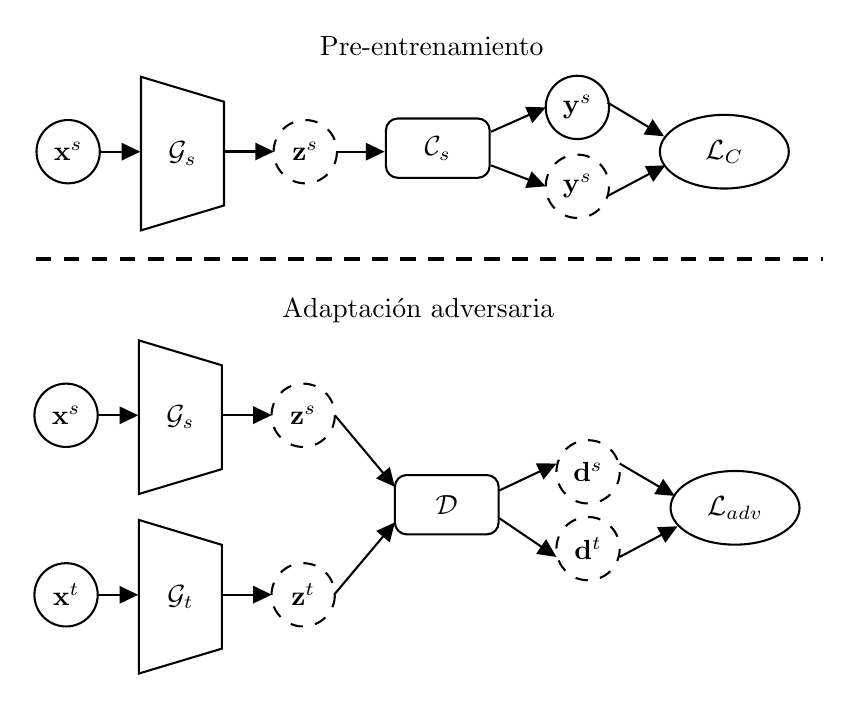
\begin{tikzpicture}[x=0.75pt,y=0.75pt,yscale=-1,xscale=1]
    %uncomment if require: \path (0,385); %set diagram left start at 0, and has height of 385

    \draw   (20.33,88.25) .. controls (20.33,79.83) and (27.16,73) .. (35.58,73) .. controls (44.01,73) and (50.83,79.83) .. (50.83,88.25) .. controls (50.83,96.67) and (44.01,103.5) .. (35.58,103.5) .. controls (27.16,103.5) and (20.33,96.67) .. (20.33,88.25) -- cycle ;

    \draw   (70.67,52.17) -- (110.67,64.17) -- (110.67,114.17) -- (70.67,126.17) -- cycle ;
    \draw    (50.83,88.25) -- (67.33,88.25) ;
    \draw [shift={(70.33,88.25)}, rotate = 180] [fill={rgb, 255:red, 0; green, 0; blue, 0 }  ][line width=0.08]  [draw opacity=0] (8.93,-4.29) -- (0,0) -- (8.93,4.29) -- cycle    ;
    \draw  [dash pattern={on 4.5pt off 4.5pt}] (134.58,88.25) .. controls (134.58,79.83) and (141.41,73) .. (149.83,73) .. controls (158.26,73) and (165.08,79.83) .. (165.08,88.25) .. controls (165.08,96.67) and (158.26,103.5) .. (149.83,103.5) .. controls (141.41,103.5) and (134.58,96.67) .. (134.58,88.25) -- cycle ;

    \draw   (188.67,77.98) .. controls (188.67,74.82) and (191.23,72.26) .. (194.38,72.26) -- (232.95,72.26) .. controls (236.11,72.26) and (238.67,74.82) .. (238.67,77.98) -- (238.67,95.12) .. controls (238.67,98.27) and (236.11,100.83) .. (232.95,100.83) -- (194.38,100.83) .. controls (191.23,100.83) and (188.67,98.27) .. (188.67,95.12) -- cycle ;
    \draw   (265.67,66.92) .. controls (265.67,58.49) and (272.49,51.67) .. (280.92,51.67) .. controls (289.34,51.67) and (296.17,58.49) .. (296.17,66.92) .. controls (296.17,75.34) and (289.34,82.17) .. (280.92,82.17) .. controls (272.49,82.17) and (265.67,75.34) .. (265.67,66.92) -- cycle ;
    \draw  [dash pattern={on 4.5pt off 4.5pt}] (265.67,104.92) .. controls (265.67,96.49) and (272.49,89.67) .. (280.92,89.67) .. controls (289.34,89.67) and (296.17,96.49) .. (296.17,104.92) .. controls (296.17,113.34) and (289.34,120.17) .. (280.92,120.17) .. controls (272.49,120.17) and (265.67,113.34) .. (265.67,104.92) -- cycle ;
    \draw   (320.67,88.25) .. controls (320.67,78.45) and (334.57,70.5) .. (351.73,70.5) .. controls (368.88,70.5) and (382.79,78.45) .. (382.79,88.25) .. controls (382.79,98.05) and (368.88,106) .. (351.73,106) .. controls (334.57,106) and (320.67,98.05) .. (320.67,88.25) -- cycle ;
    \draw    (111.33,88.17) -- (131.67,88.17) ;
    \draw [shift={(134.67,88.17)}, rotate = 180] [fill={rgb, 255:red, 0; green, 0; blue, 0 }  ][line width=0.08]  [draw opacity=0] (8.93,-4.29) -- (0,0) -- (8.93,4.29) -- cycle    ;
    \draw    (164.67,88.25) -- (185,88.25) ;
    \draw [shift={(188,88.25)}, rotate = 180] [fill={rgb, 255:red, 0; green, 0; blue, 0 }  ][line width=0.08]  [draw opacity=0] (8.93,-4.29) -- (0,0) -- (8.93,4.29) -- cycle    ;
    \draw    (239.33,78.64) -- (262.93,68.14) ;
    \draw [shift={(265.67,66.92)}, rotate = 156] [fill={rgb, 255:red, 0; green, 0; blue, 0 }  ][line width=0.08]  [draw opacity=0] (8.93,-4.29) -- (0,0) -- (8.93,4.29) -- cycle    ;
    \draw    (239.33,94.83) -- (262.87,103.84) ;
    \draw [shift={(265.67,104.92)}, rotate = 200.95] [fill={rgb, 255:red, 0; green, 0; blue, 0 }  ][line width=0.08]  [draw opacity=0] (8.93,-4.29) -- (0,0) -- (8.93,4.29) -- cycle    ;
    \draw    (295.5,64.58) -- (320.09,79.29) ;
    \draw [shift={(322.67,80.83)}, rotate = 210.89] [fill={rgb, 255:red, 0; green, 0; blue, 0 }  ][line width=0.08]  [draw opacity=0] (8.93,-4.29) -- (0,0) -- (8.93,4.29) -- cycle    ;
    \draw    (295.5,109.58) -- (320.68,96.24) ;
    \draw [shift={(323.33,94.83)}, rotate = 152.08] [fill={rgb, 255:red, 0; green, 0; blue, 0 }  ][line width=0.08]  [draw opacity=0] (8.93,-4.29) -- (0,0) -- (8.93,4.29) -- cycle    ;
    \draw   (19.33,215.25) .. controls (19.33,206.83) and (26.16,200) .. (34.58,200) .. controls (43.01,200) and (49.83,206.83) .. (49.83,215.25) .. controls (49.83,223.67) and (43.01,230.5) .. (34.58,230.5) .. controls (26.16,230.5) and (19.33,223.67) .. (19.33,215.25) -- cycle ;

    \draw   (69.67,179.17) -- (109.67,191.17) -- (109.67,241.17) -- (69.67,253.17) -- cycle ;
    \draw    (49.83,215.25) -- (66.33,215.25) ;
    \draw [shift={(69.33,215.25)}, rotate = 180] [fill={rgb, 255:red, 0; green, 0; blue, 0 }  ][line width=0.08]  [draw opacity=0] (8.93,-4.29) -- (0,0) -- (8.93,4.29) -- cycle    ;
    \draw  [dash pattern={on 4.5pt off 4.5pt}] (133.58,215.25) .. controls (133.58,206.83) and (140.41,200) .. (148.83,200) .. controls (157.26,200) and (164.08,206.83) .. (164.08,215.25) .. controls (164.08,223.67) and (157.26,230.5) .. (148.83,230.5) .. controls (140.41,230.5) and (133.58,223.67) .. (133.58,215.25) -- cycle ;

    \draw    (110.33,215.17) -- (130.67,215.17) ;
    \draw [shift={(133.67,215.17)}, rotate = 180] [fill={rgb, 255:red, 0; green, 0; blue, 0 }  ][line width=0.08]  [draw opacity=0] (8.93,-4.29) -- (0,0) -- (8.93,4.29) -- cycle    ;
    \draw    (164.08,215.25) -- (191.07,247.45) ;
    \draw [shift={(193,249.75)}, rotate = 230.03] [fill={rgb, 255:red, 0; green, 0; blue, 0 }  ][line width=0.08]  [draw opacity=0] (8.93,-4.29) -- (0,0) -- (8.93,4.29) -- cycle    ;
    \draw   (19.33,301.75) .. controls (19.33,293.33) and (26.16,286.5) .. (34.58,286.5) .. controls (43.01,286.5) and (49.83,293.33) .. (49.83,301.75) .. controls (49.83,310.17) and (43.01,317) .. (34.58,317) .. controls (26.16,317) and (19.33,310.17) .. (19.33,301.75) -- cycle ;

    \draw   (69.67,265.67) -- (109.67,277.67) -- (109.67,327.67) -- (69.67,339.67) -- cycle ;
    \draw    (49.83,301.75) -- (66.33,301.75) ;
    \draw [shift={(69.33,301.75)}, rotate = 180] [fill={rgb, 255:red, 0; green, 0; blue, 0 }  ][line width=0.08]  [draw opacity=0] (8.93,-4.29) -- (0,0) -- (8.93,4.29) -- cycle    ;
    \draw  [dash pattern={on 4.5pt off 4.5pt}] (133.58,301.75) .. controls (133.58,293.33) and (140.41,286.5) .. (148.83,286.5) .. controls (157.26,286.5) and (164.08,293.33) .. (164.08,301.75) .. controls (164.08,310.17) and (157.26,317) .. (148.83,317) .. controls (140.41,317) and (133.58,310.17) .. (133.58,301.75) -- cycle ;
    \draw    (110.33,301.67) -- (130.67,301.67) ;
    \draw [shift={(133.67,301.67)}, rotate = 180] [fill={rgb, 255:red, 0; green, 0; blue, 0 }  ][line width=0.08]  [draw opacity=0] (8.93,-4.29) -- (0,0) -- (8.93,4.29) -- cycle    ;
    \draw    (163.67,301.75) -- (191.07,269.19) ;
    \draw [shift={(193,266.89)}, rotate = 130.08] [fill={rgb, 255:red, 0; green, 0; blue, 0 }  ][line width=0.08]  [draw opacity=0] (8.93,-4.29) -- (0,0) -- (8.93,4.29) -- cycle    ;
    \draw   (193,249.75) .. controls (193,246.59) and (195.56,244.04) .. (198.71,244.04) -- (237.29,244.04) .. controls (240.44,244.04) and (243,246.59) .. (243,249.75) -- (243,266.89) .. controls (243,270.05) and (240.44,272.61) .. (237.29,272.61) -- (198.71,272.61) .. controls (195.56,272.61) and (193,270.05) .. (193,266.89) -- cycle ;

    \draw  [dash pattern={on 4.5pt off 4.5pt}] (270.83,242.5) .. controls (270.83,234.08) and (277.66,227.25) .. (286.08,227.25) .. controls (294.51,227.25) and (301.33,234.08) .. (301.33,242.5) .. controls (301.33,250.92) and (294.51,257.75) .. (286.08,257.75) .. controls (277.66,257.75) and (270.83,250.92) .. (270.83,242.5) -- cycle ;

    \draw  [dash pattern={on 4.5pt off 4.5pt}] (270.83,279.5) .. controls (270.83,271.08) and (277.66,264.25) .. (286.08,264.25) .. controls (294.51,264.25) and (301.33,271.08) .. (301.33,279.5) .. controls (301.33,287.92) and (294.51,294.75) .. (286.08,294.75) .. controls (277.66,294.75) and (270.83,287.92) .. (270.83,279.5) -- cycle ;

    \draw   (325.83,259.83) .. controls (325.83,250.03) and (339.74,242.08) .. (356.9,242.08) .. controls (374.05,242.08) and (387.96,250.03) .. (387.96,259.83) .. controls (387.96,269.64) and (374.05,277.58) .. (356.9,277.58) .. controls (339.74,277.58) and (325.83,269.64) .. (325.83,259.83) -- cycle ;

    \draw    (243.17,251.56) -- (268.12,239.78) ;
    \draw [shift={(270.83,238.5)}, rotate = 154.73] [fill={rgb, 255:red, 0; green, 0; blue, 0 }  ][line width=0.08]  [draw opacity=0] (8.93,-4.29) -- (0,0) -- (8.93,4.29) -- cycle    ;
    \draw    (243.17,264.75) -- (268.35,281.82) ;
    \draw [shift={(270.83,283.5)}, rotate = 214.13] [fill={rgb, 255:red, 0; green, 0; blue, 0 }  ][line width=0.08]  [draw opacity=0] (8.93,-4.29) -- (0,0) -- (8.93,4.29) -- cycle    ;
    \draw    (301.33,238.5) -- (325.25,252.56) ;
    \draw [shift={(327.83,254.08)}, rotate = 210.46] [fill={rgb, 255:red, 0; green, 0; blue, 0 }  ][line width=0.08]  [draw opacity=0] (8.93,-4.29) -- (0,0) -- (8.93,4.29) -- cycle    ;
    \draw    (301.33,283.5) -- (326.52,270.15) ;
    \draw [shift={(329.17,268.75)}, rotate = 152.08] [fill={rgb, 255:red, 0; green, 0; blue, 0 }  ][line width=0.08]  [draw opacity=0] (8.93,-4.29) -- (0,0) -- (8.93,4.29) -- cycle    ;
    \draw [line width=1.5]  [dash pattern={on 5.63pt off 4.5pt}]  (20,140) -- (399.5,140) ;

    \draw (280.92,66.92) node   [align=left] {\begin{minipage}[lt]{21.08pt}\setlength\topsep{0pt}
        \begin{center}
          $\mathbf{y}^s$
        \end{center}
      \end{minipage}};
    \draw (280.92,104.92) node   [align=left] {\begin{minipage}[lt]{21.08pt}\setlength\topsep{0pt}
        \begin{center}
          $\mathbf{y}^s$
        \end{center}
      \end{minipage}};
    \draw (351.73,88.25) node   [align=left] {\begin{minipage}[lt]{32.64pt}\setlength\topsep{0pt}
        \begin{center}
          $\mathcal{L}_C$
        \end{center}
      \end{minipage}};
    \draw (149.83,88.25) node   [align=left] {\begin{minipage}[lt]{21.08pt}\setlength\topsep{0pt}
        \begin{center}
          $\mathbf{z}^s$
        \end{center}
      \end{minipage}};
    \draw (35.58,88.25) node   [align=left] {\begin{minipage}[lt]{21.08pt}\setlength\topsep{0pt}
        \begin{center}
          $\mathbf{x}^s$
        \end{center}
      \end{minipage}};
    \draw (90.67,89.17) node   [align=left] {\begin{minipage}[lt]{22.78pt}\setlength\topsep{0pt}
        \begin{center}
          $\mathcal{G}_s$
        \end{center}
      \end{minipage}};
    \draw (213.67,86.73) node   [align=left] {\begin{minipage}[lt]{26.23pt}\setlength\topsep{0pt}
        \begin{center}
          $\mathcal{C}_s$
        \end{center}
      \end{minipage}};
    \draw (89.67,216.17) node   [align=left] {\begin{minipage}[lt]{22.78pt}\setlength\topsep{0pt}
        \begin{center}
          $\mathcal{G}_s$
        \end{center}
      \end{minipage}};
    \draw (148.83,215.25) node   [align=left] {\begin{minipage}[lt]{21.08pt}\setlength\topsep{0pt}
        \begin{center}
          $\mathbf{z}^s$
        \end{center}
      \end{minipage}};
    \draw (34.58,215.25) node   [align=left] {\begin{minipage}[lt]{21.08pt}\setlength\topsep{0pt}
        \begin{center}
          $\mathbf{x}^s$
        \end{center}
      \end{minipage}};
    \draw (89.67,302.67) node   [align=left] {\begin{minipage}[lt]{22.78pt}\setlength\topsep{0pt}
        \begin{center}
          $\mathcal{G}_t$
        \end{center}
      \end{minipage}};
    \draw (34.58,301.75) node   [align=left] {\begin{minipage}[lt]{21.08pt}\setlength\topsep{0pt}
        \begin{center}
          $\mathbf{x}^t$
        \end{center}
      \end{minipage}};
    \draw (148.83,301.75) node   [align=left] {\begin{minipage}[lt]{21.08pt}\setlength\topsep{0pt}
        \begin{center}
          $\mathbf{z}^t$
        \end{center}
      \end{minipage}};
    \draw (218,258.5) node   [align=left] {\begin{minipage}[lt]{26.23pt}\setlength\topsep{0pt}
        \begin{center}
          $\mathcal{D}$
        \end{center}
      \end{minipage}};
    \draw (356.9,259.83) node   [align=left] {\begin{minipage}[lt]{32.64pt}\setlength\topsep{0pt}
        \begin{center}
          $\mathcal{L}_{adv}$
        \end{center}
      \end{minipage}};
    \draw (286.08,279.5) node   [align=left] {\begin{minipage}[lt]{21.08pt}\setlength\topsep{0pt}
        \begin{center}
          $\mathbf{d}^t$
        \end{center}
      \end{minipage}};
    \draw (286.08,242.5) node   [align=left] {\begin{minipage}[lt]{21.08pt}\setlength\topsep{0pt}
        \begin{center}
          $\mathbf{d}^s$
        \end{center}
      \end{minipage}};
    \draw (210.75,37.5) node   [align=left] {\begin{minipage}[lt]{258.06pt}\setlength\topsep{0pt}
        \begin{center}
          Pre-entrenamiento
        \end{center}
      \end{minipage}};
    \draw (204.25,165) node   [align=left] {\begin{minipage}[lt]{266.22pt}\setlength\topsep{0pt}
        \begin{center}
          Adaptación adversaria
        \end{center}
      \end{minipage}};

  \end{tikzpicture}
  \caption[Esquema de {\it ADDA}]{Esquema de las {\it ADDA}. Los supra indices $s$ y $t$ indican si los datos son del origen o destino respectivamente.
    Los círculos con líneas rayadas son salidas de los modelos mientras que los círculos de líneas sólidas son datos conocidos.
    La primera fase consta de un pre-entrenamiento con una red generadora $\mathcal{G}_s$ con los datos origen y la segunda fase de adaptación
    consta de otra red generadora $\mathcal{G}_t$ que debe aprender a generar el mismo espacio latente que $\mathcal{G}_s$ con los datos de destino para confundir a $\mathcal{D}$.}
  \label{fig:adda-esquema}
\end{figure}

No obstante del cambio, los objetivos de {\it ADDA} son similares a los de las {\it DANN} a excepción de
$\mathcal{G}_t$. La ecuación \ref{eq:adda-loss-clasificadora} contiene $\mathcal{L}_\mathcal{C}$ que es análoga a
\ref{eq:dann-loss-clasificadora}. La ecuación \ref{eq:adda-loss-discriminadora} contiene $\mathcal{L}_{adv}$ que es
análoga a \ref{eq:dann-loss-discriminadora}. Finalmente, la ecuación \ref{eq:adda-objetivo} contiene el objetivo a
optimizar que asigna gradientes pequeños a registros de destino que sean similares a los de origen y gradientes mas
grandes para los otros registros de destino.

\begin{align}
   & \min_{\mathcal{G}_s, \mathcal{C}} \mathcal{L}_\mathcal{C}(\mathbf{x}^s, \mathbf{y}^s)                                                            = \mathcal{L}_{CE}(C_s(\mathcal{G}_s(\mathbf{x}^s)), \mathbf{y}^s)
  \label{eq:adda-loss-clasificadora}                                                                                                                                                                                                                                                                                                                                                          \\
   & \max_{\mathcal{D}} \mathcal{L}_{adv}(\mathbf{x}^s, \mathbf{x}^t)                                                                                 = \mathbb{E}_{\mathbf{x}^s \sim \mathcal{\hat{S}}}\log[\mathcal{D}(\mathcal{G}_s(\mathbf{x}^s))] + \mathbb{E}_{\mathbf{x}^t \sim \mathcal{\hat{T}}}\log[1-\mathcal{D}(\mathcal{G}_t(\mathbf{x}^t))] \label{eq:adda-loss-discriminadora} \\
   & \min_{\mathcal{G}_t} - \mathbb{E}_{\mathbf{x}^t \sim \mathcal{\hat{T}}} \log[\mathcal{D}(\mathcal{G}_t(\mathbf{x}^t))]  \label{eq:adda-objetivo}
\end{align}

\subsection{Batch Spectral Penalization}

Aunque los metodos de adaptación de dominio adversarios mejoran la {\it transferibilidad} de las características
aprendidas; es decir, la capacidad de que las representaciones puedan superar las discrepancias entre los dominios, lo
hacen a costa de la {\it discriminabilidad}; es decir, la facilidad de separar categorias sobre las representaciones de
ambos dominios \parencite{chen2019transferability}. Al aplicar descomposición en valores singulares ({\it SVD} en inglés) para analizar
las propiedades espectrales de las representaciones aprendidas en batches, se confirma que los eigenvectors con valores
singulares más altos dominan la {\it transferibilidad} mientras que los eigenvectors con valores singulares más
pequeños se encuentran penalizados, lo que provoca una {\it discriminabilidad} deficiente. {\it Batch Spectral
    Penalization} {\it BSP} \parencite{chen2019transferability} penaliza el mayor valor singular para que los demás eigenvectors puedan mejorar la {\it
    discriminabilidad}. $\mathcal{L}_{BSP}$ es propuesto como un término de regularización sobre los $k$ mayores valores
singulares:

\begin{align}
  \mathcal{L}_{BSP}(\mathbf{z}) = \sum_{i=0}^{k} (\sigma_{s, i}^2 + \sigma_{t, i}^2)
  \label{eq:bsp}
\end{align}

Donde $\sigma_{s, i}$ y $\sigma_{t, i}$ corresponden al $i$-ésimo mayor valor singular de $\Sigma_s$ y $\Sigma_t$
respectivamente. En la presente tesis se utilizará $k=1$.

  {\it BSP} puede integrarse a cualquiera de los esquemas mencionados anteriormente, por ejemplo a una {\it DANN} (figura \ref{fig:bsp-esquema-dann}).

\begin{figure}[H]
  \centering

  \tikzset{every picture/.style={line width=0.75pt}} %set default line width to 0.75pt        

  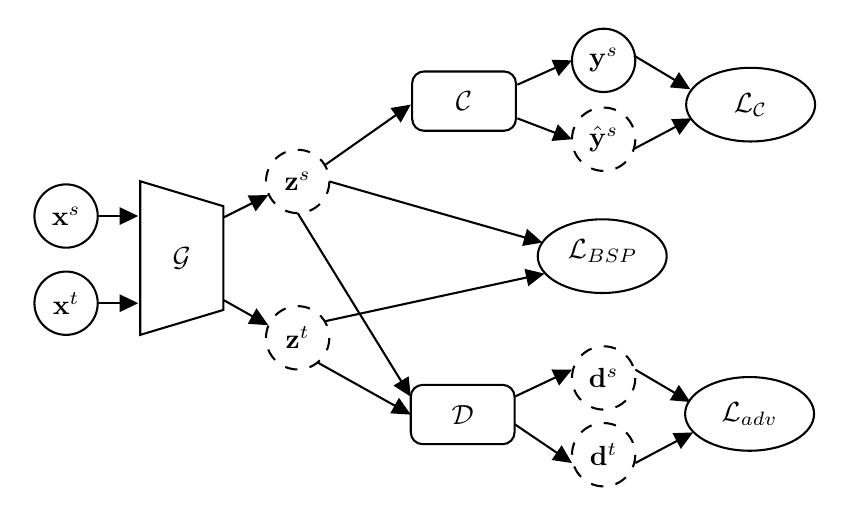
\begin{tikzpicture}[x=0.75pt,y=0.75pt,yscale=-1,xscale=1]
    %uncomment if require: \path (0,300); %set diagram left start at 0, and has height of 300

    %Shape: Circle [id:dp14395415737572304] 
    \draw   (57,126.75) .. controls (57,118.33) and (63.83,111.5) .. (72.25,111.5) .. controls (80.67,111.5) and (87.5,118.33) .. (87.5,126.75) .. controls (87.5,135.17) and (80.67,142) .. (72.25,142) .. controls (63.83,142) and (57,135.17) .. (57,126.75) -- cycle ;

    %Shape: Circle [id:dp5294927781460403] 
    \draw   (57,168.75) .. controls (57,160.33) and (63.83,153.5) .. (72.25,153.5) .. controls (80.67,153.5) and (87.5,160.33) .. (87.5,168.75) .. controls (87.5,177.17) and (80.67,184) .. (72.25,184) .. controls (63.83,184) and (57,177.17) .. (57,168.75) -- cycle ;

    %Shape: Trapezoid [id:dp3621515034386269] 
    \draw   (108,110) -- (148,122) -- (148,172) -- (108,184) -- cycle ;

    %Straight Lines [id:da711615291035981] 
    \draw    (87.5,126.75) -- (104,126.75) ;
    \draw [shift={(107,126.75)}, rotate = 180] [fill={rgb, 255:red, 0; green, 0; blue, 0 }  ][line width=0.08]  [draw opacity=0] (8.93,-4.29) -- (0,0) -- (8.93,4.29) -- cycle    ;
    %Shape: Circle [id:dp5854711906138592] 
    \draw  [dash pattern={on 4.5pt off 4.5pt}] (168.58,110.08) .. controls (168.58,101.66) and (175.41,94.83) .. (183.83,94.83) .. controls (192.26,94.83) and (199.08,101.66) .. (199.08,110.08) .. controls (199.08,118.51) and (192.26,125.33) .. (183.83,125.33) .. controls (175.41,125.33) and (168.58,118.51) .. (168.58,110.08) -- cycle ;

    %Shape: Circle [id:dp8402316163188099] 
    \draw  [dash pattern={on 4.5pt off 4.5pt}] (168.58,185.42) .. controls (168.58,176.99) and (175.41,170.17) .. (183.83,170.17) .. controls (192.26,170.17) and (199.08,176.99) .. (199.08,185.42) .. controls (199.08,193.84) and (192.26,200.67) .. (183.83,200.67) .. controls (175.41,200.67) and (168.58,193.84) .. (168.58,185.42) -- cycle ;

    %Rounded Rect [id:dp15165955457538138] 
    \draw   (239,62.81) .. controls (239,59.65) and (241.56,57.1) .. (244.71,57.1) -- (283.29,57.1) .. controls (286.44,57.1) and (289,59.65) .. (289,62.81) -- (289,79.95) .. controls (289,83.11) and (286.44,85.67) .. (283.29,85.67) -- (244.71,85.67) .. controls (241.56,85.67) and (239,83.11) .. (239,79.95) -- cycle ;

    %Rounded Rect [id:dp47289041628378614] 
    \draw   (238.33,213.81) .. controls (238.33,210.65) and (240.89,208.1) .. (244.05,208.1) -- (282.62,208.1) .. controls (285.77,208.1) and (288.33,210.65) .. (288.33,213.81) -- (288.33,230.95) .. controls (288.33,234.11) and (285.77,236.67) .. (282.62,236.67) -- (244.05,236.67) .. controls (240.89,236.67) and (238.33,234.11) .. (238.33,230.95) -- cycle ;

    %Shape: Circle [id:dp20484409800302994] 
    \draw  [dash pattern={on 4.5pt off 4.5pt}] (316,204.75) .. controls (316,196.33) and (322.83,189.5) .. (331.25,189.5) .. controls (339.67,189.5) and (346.5,196.33) .. (346.5,204.75) .. controls (346.5,213.17) and (339.67,220) .. (331.25,220) .. controls (322.83,220) and (316,213.17) .. (316,204.75) -- cycle ;

    %Shape: Circle [id:dp19954579063976796] 
    \draw  [dash pattern={on 4.5pt off 4.5pt}] (316,241.75) .. controls (316,233.33) and (322.83,226.5) .. (331.25,226.5) .. controls (339.67,226.5) and (346.5,233.33) .. (346.5,241.75) .. controls (346.5,250.17) and (339.67,257) .. (331.25,257) .. controls (322.83,257) and (316,250.17) .. (316,241.75) -- cycle ;

    %Shape: Ellipse [id:dp41632665310072503] 
    \draw   (370.5,222.08) .. controls (370.5,212.28) and (384.41,204.33) .. (401.56,204.33) .. controls (418.72,204.33) and (432.63,212.28) .. (432.63,222.08) .. controls (432.63,231.89) and (418.72,239.83) .. (401.56,239.83) .. controls (384.41,239.83) and (370.5,231.89) .. (370.5,222.08) -- cycle ;

    %Shape: Circle [id:dp17102829278099274] 
    \draw   (316,51.75) .. controls (316,43.33) and (322.83,36.5) .. (331.25,36.5) .. controls (339.67,36.5) and (346.5,43.33) .. (346.5,51.75) .. controls (346.5,60.17) and (339.67,67) .. (331.25,67) .. controls (322.83,67) and (316,60.17) .. (316,51.75) -- cycle ;
    %Shape: Circle [id:dp2918994940011912] 
    \draw  [dash pattern={on 4.5pt off 4.5pt}] (316,89.75) .. controls (316,81.33) and (322.83,74.5) .. (331.25,74.5) .. controls (339.67,74.5) and (346.5,81.33) .. (346.5,89.75) .. controls (346.5,98.17) and (339.67,105) .. (331.25,105) .. controls (322.83,105) and (316,98.17) .. (316,89.75) -- cycle ;
    %Shape: Ellipse [id:dp7208514036481783] 
    \draw   (371,73.08) .. controls (371,63.28) and (384.91,55.33) .. (402.06,55.33) .. controls (419.22,55.33) and (433.13,63.28) .. (433.13,73.08) .. controls (433.13,82.89) and (419.22,90.83) .. (402.06,90.83) .. controls (384.91,90.83) and (371,82.89) .. (371,73.08) -- cycle ;
    %Straight Lines [id:da35699780719749463] 
    \draw    (87.5,168.75) -- (104,168.75) ;
    \draw [shift={(107,168.75)}, rotate = 180] [fill={rgb, 255:red, 0; green, 0; blue, 0 }  ][line width=0.08]  [draw opacity=0] (8.93,-4.29) -- (0,0) -- (8.93,4.29) -- cycle    ;
    %Straight Lines [id:da18773339124658595] 
    \draw    (148.33,127.33) -- (166.98,118.01) ;
    \draw [shift={(169.67,116.67)}, rotate = 153.43] [fill={rgb, 255:red, 0; green, 0; blue, 0 }  ][line width=0.08]  [draw opacity=0] (8.93,-4.29) -- (0,0) -- (8.93,4.29) -- cycle    ;
    %Straight Lines [id:da22178069673434142] 
    \draw    (148.33,167.33) -- (167.05,177.86) ;
    \draw [shift={(169.67,179.33)}, rotate = 209.36] [fill={rgb, 255:red, 0; green, 0; blue, 0 }  ][line width=0.08]  [draw opacity=0] (8.93,-4.29) -- (0,0) -- (8.93,4.29) -- cycle    ;
    %Straight Lines [id:da7263329854343115] 
    \draw    (197.25,102) -- (235.88,74.81) ;
    \draw [shift={(238.33,73.08)}, rotate = 144.86] [fill={rgb, 255:red, 0; green, 0; blue, 0 }  ][line width=0.08]  [draw opacity=0] (8.93,-4.29) -- (0,0) -- (8.93,4.29) -- cycle    ;
    %Straight Lines [id:da5895896069004276] 
    \draw    (193.6,197.4) -- (235.71,220.95) ;
    \draw [shift={(238.33,222.42)}, rotate = 209.22] [fill={rgb, 255:red, 0; green, 0; blue, 0 }  ][line width=0.08]  [draw opacity=0] (8.93,-4.29) -- (0,0) -- (8.93,4.29) -- cycle    ;
    %Straight Lines [id:da504234275800213] 
    \draw    (183.83,125.33) -- (236.76,211.26) ;
    \draw [shift={(238.33,213.81)}, rotate = 238.37] [fill={rgb, 255:red, 0; green, 0; blue, 0 }  ][line width=0.08]  [draw opacity=0] (8.93,-4.29) -- (0,0) -- (8.93,4.29) -- cycle    ;
    %Straight Lines [id:da10127819240633107] 
    \draw    (288.33,213.81) -- (313.29,202.03) ;
    \draw [shift={(316,200.75)}, rotate = 154.73] [fill={rgb, 255:red, 0; green, 0; blue, 0 }  ][line width=0.08]  [draw opacity=0] (8.93,-4.29) -- (0,0) -- (8.93,4.29) -- cycle    ;
    %Straight Lines [id:da18118282714853473] 
    \draw    (288.33,227) -- (313.52,244.07) ;
    \draw [shift={(316,245.75)}, rotate = 214.13] [fill={rgb, 255:red, 0; green, 0; blue, 0 }  ][line width=0.08]  [draw opacity=0] (8.93,-4.29) -- (0,0) -- (8.93,4.29) -- cycle    ;
    %Straight Lines [id:da46435990995985477] 
    \draw    (346.5,200.75) -- (370.41,214.81) ;
    \draw [shift={(373,216.33)}, rotate = 210.46] [fill={rgb, 255:red, 0; green, 0; blue, 0 }  ][line width=0.08]  [draw opacity=0] (8.93,-4.29) -- (0,0) -- (8.93,4.29) -- cycle    ;
    %Straight Lines [id:da3066500527802958] 
    \draw    (346.5,245.75) -- (371.68,232.4) ;
    \draw [shift={(374.33,231)}, rotate = 152.08] [fill={rgb, 255:red, 0; green, 0; blue, 0 }  ][line width=0.08]  [draw opacity=0] (8.93,-4.29) -- (0,0) -- (8.93,4.29) -- cycle    ;
    %Straight Lines [id:da9357957653419868] 
    \draw    (289.67,63.48) -- (313.26,52.97) ;
    \draw [shift={(316,51.75)}, rotate = 156] [fill={rgb, 255:red, 0; green, 0; blue, 0 }  ][line width=0.08]  [draw opacity=0] (8.93,-4.29) -- (0,0) -- (8.93,4.29) -- cycle    ;
    %Straight Lines [id:da5822336916421971] 
    \draw    (289.67,79.67) -- (313.2,88.68) ;
    \draw [shift={(316,89.75)}, rotate = 200.95] [fill={rgb, 255:red, 0; green, 0; blue, 0 }  ][line width=0.08]  [draw opacity=0] (8.93,-4.29) -- (0,0) -- (8.93,4.29) -- cycle    ;
    %Straight Lines [id:da8400721166176619] 
    \draw    (345.83,49.42) -- (370.43,64.13) ;
    \draw [shift={(373,65.67)}, rotate = 210.89] [fill={rgb, 255:red, 0; green, 0; blue, 0 }  ][line width=0.08]  [draw opacity=0] (8.93,-4.29) -- (0,0) -- (8.93,4.29) -- cycle    ;
    %Straight Lines [id:da5048948243554285] 
    \draw    (345.83,94.42) -- (371.02,81.07) ;
    \draw [shift={(373.67,79.67)}, rotate = 152.08] [fill={rgb, 255:red, 0; green, 0; blue, 0 }  ][line width=0.08]  [draw opacity=0] (8.93,-4.29) -- (0,0) -- (8.93,4.29) -- cycle    ;
    %Shape: Ellipse [id:dp8464659325338855] 
    \draw   (299.5,146.08) .. controls (299.5,136.28) and (313.41,128.33) .. (330.56,128.33) .. controls (347.72,128.33) and (361.63,136.28) .. (361.63,146.08) .. controls (361.63,155.89) and (347.72,163.83) .. (330.56,163.83) .. controls (313.41,163.83) and (299.5,155.89) .. (299.5,146.08) -- cycle ;
    %Straight Lines [id:da5523565128759309] 
    \draw    (197.2,177.4) -- (299.82,155.14) ;
    \draw [shift={(302.75,154.5)}, rotate = 167.76] [fill={rgb, 255:red, 0; green, 0; blue, 0 }  ][line width=0.08]  [draw opacity=0] (8.93,-4.29) -- (0,0) -- (8.93,4.29) -- cycle    ;
    %Straight Lines [id:da24838256047555873] 
    \draw    (199.08,110.08) -- (298.87,138.67) ;
    \draw [shift={(301.75,139.5)}, rotate = 195.99] [fill={rgb, 255:red, 0; green, 0; blue, 0 }  ][line width=0.08]  [draw opacity=0] (8.93,-4.29) -- (0,0) -- (8.93,4.29) -- cycle    ;

    % Text Node
    \draw (331.25,51.75) node   [align=left] {\begin{minipage}[lt]{21.08pt}\setlength\topsep{0pt}
        \begin{center}
          $\mathbf{y}^s$
        \end{center}

      \end{minipage}};
    % Text Node
    \draw (331.25,89.75) node   [align=left] {\begin{minipage}[lt]{21.08pt}\setlength\topsep{0pt}
        \begin{center}
          $\hat{\mathbf{y}}^s$
        \end{center}

      \end{minipage}};
    % Text Node
    \draw (402.06,73.08) node   [align=left] {\begin{minipage}[lt]{32.64pt}\setlength\topsep{0pt}
        \begin{center}
          $\mathcal{L}_{\mathcal{C}}$
        \end{center}

      \end{minipage}};
    % Text Node
    \draw (401.56,222.08) node   [align=left] {\begin{minipage}[lt]{32.64pt}\setlength\topsep{0pt}
        \begin{center}
          $\mathcal{L}_{adv}$
        \end{center}

      \end{minipage}};
    % Text Node
    \draw (331.25,241.75) node   [align=left] {\begin{minipage}[lt]{21.08pt}\setlength\topsep{0pt}
        \begin{center}
          $\mathbf{d}^t$
        \end{center}

      \end{minipage}};
    % Text Node
    \draw (331.25,204.75) node   [align=left] {\begin{minipage}[lt]{21.08pt}\setlength\topsep{0pt}
        \begin{center}
          $\mathbf{d}^s$
        \end{center}

      \end{minipage}};
    % Text Node
    \draw (263.33,222.56) node   [align=left] {\begin{minipage}[lt]{26.23pt}\setlength\topsep{0pt}
        \begin{center}
          $\mathcal{D}$
        \end{center}

      \end{minipage}};
    % Text Node
    \draw (264,71.56) node   [align=left] {\begin{minipage}[lt]{26.23pt}\setlength\topsep{0pt}
        \begin{center}
          $\mathcal{C}$
        \end{center}

      \end{minipage}};
    % Text Node
    \draw (183.83,185.42) node   [align=left] {\begin{minipage}[lt]{21.08pt}\setlength\topsep{0pt}
        \begin{center}
          $\mathbf{z}^t$
        \end{center}

      \end{minipage}};
    % Text Node
    \draw (183.83,110.08) node   [align=left] {\begin{minipage}[lt]{21.08pt}\setlength\topsep{0pt}
        \begin{center}
          $\mathbf{z}^s$
        \end{center}

      \end{minipage}};
    % Text Node
    \draw (128,147) node   [align=left] {\begin{minipage}[lt]{22.78pt}\setlength\topsep{0pt}
        \begin{center}
          $\mathcal{G}$
        \end{center}

      \end{minipage}};
    % Text Node
    \draw (72.25,168.75) node   [align=left] {\begin{minipage}[lt]{21.08pt}\setlength\topsep{0pt}
        \begin{center}
          $\mathbf{x}^t$
        \end{center}

      \end{minipage}};
    % Text Node
    \draw (72.25,126.75) node   [align=left] {\begin{minipage}[lt]{21.08pt}\setlength\topsep{0pt}
        \begin{center}
          $\mathbf{x}^s$
        \end{center}

      \end{minipage}};
    % Text Node
    \draw (312.5,136.4) node [anchor=north west][inner sep=0.75pt]    {$\mathcal{L}_{BSP} $};

  \end{tikzpicture}

  \caption[Esquema de {\it DANN+BSP}]{Esquema de un modelo {\it DANN+BSP}.}
  \label{fig:bsp-esquema-dann}
\end{figure}

Por lo tanto, un modelo {\it DANN+BSP} presenta como objetivos:

\begin{align}
   & \min_{\mathcal{G},\mathcal{C}} \mathcal{L}_\mathcal{C}(\mathbf{x}^s, \mathbf{y}^s) + \lambda \mathcal{L}_{adv}(\mathbf{x}^s, \mathbf{x}^t) + \beta \mathcal{L}_{BSP}(\mathcal{G}(\mathbf{x})) \\
   & \max_{\mathcal{D}} \mathcal{L}_{adv}(\mathbf{x}^s, \mathbf{x}^t)
  \label{eq:bsp-dann-obejtivo}
\end{align}

Donde $\beta$ es el parámetro que regula el trade-off de $\mathcal{L}_{BSP}$.

\subsection{Margin Disparity Discrepancy}

Las técnicas detalladas hasta el momento implican algoritmos de optimización minimax, que funcionan correctamente en
los métodos basados en el aprendizaje adversario. Sin embargo, estos algoritmos utilizan funciones de scoreo que
carecen de garantías teóricas ya que se estudiaron funciones de pérdida 0-1. Es por esto que se introducen métodos que
apuntan a reducir la brecha que existe entre la teoría y el algoritmo, como Margin Disparity Discrepancy {\it MDD} \parencite{zhang2019bridging}. La idea general de {\it MDD} es introducir una segunda red clasificadora $\mathcal{C}^{'}$ y
relacionar su salida con la de $\mathcal{C}$.

\begin{figure}[H]
  \centering

  \tikzset{every picture/.style={line width=0.75pt}} %set default line width to 0.75pt        

  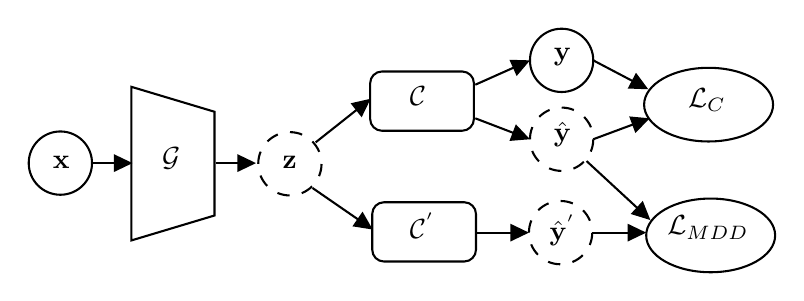
\begin{tikzpicture}[x=0.75pt,y=0.75pt,yscale=-1,xscale=1]
    %uncomment if require: \path (0,424); %set diagram left start at 0, and has height of 424

    %Shape: Circle [id:dp37402229817841603] 
    \draw   (60.5,104.75) .. controls (60.5,96.33) and (67.33,89.5) .. (75.75,89.5) .. controls (84.17,89.5) and (91,96.33) .. (91,104.75) .. controls (91,113.17) and (84.17,120) .. (75.75,120) .. controls (67.33,120) and (60.5,113.17) .. (60.5,104.75) -- cycle ;
    %Shape: Trapezoid [id:dp5518581764728496] 
    \draw   (110,68) -- (150,80) -- (150,130) -- (110,142) -- cycle ;
    %Straight Lines [id:da7900111351501842] 
    \draw    (91,104.75) -- (107.5,104.75) ;
    \draw [shift={(110.5,104.75)}, rotate = 180] [fill={rgb, 255:red, 0; green, 0; blue, 0 }  ][line width=0.08]  [draw opacity=0] (8.93,-4.29) -- (0,0) -- (8.93,4.29) -- cycle    ;
    %Shape: Circle [id:dp6237032464701955] 
    \draw  [dash pattern={on 4.5pt off 4.5pt}] (171.08,105.08) .. controls (171.08,96.66) and (177.91,89.83) .. (186.33,89.83) .. controls (194.76,89.83) and (201.58,96.66) .. (201.58,105.08) .. controls (201.58,113.51) and (194.76,120.33) .. (186.33,120.33) .. controls (177.91,120.33) and (171.08,113.51) .. (171.08,105.08) -- cycle ;
    %Rounded Rect [id:dp17455651105714143] 
    \draw   (225,66.31) .. controls (225,63.15) and (227.56,60.6) .. (230.71,60.6) -- (269.29,60.6) .. controls (272.44,60.6) and (275,63.15) .. (275,66.31) -- (275,83.45) .. controls (275,86.61) and (272.44,89.17) .. (269.29,89.17) -- (230.71,89.17) .. controls (227.56,89.17) and (225,86.61) .. (225,83.45) -- cycle ;
    %Shape: Circle [id:dp2140151642409336] 
    \draw   (302,55.25) .. controls (302,46.83) and (308.83,40) .. (317.25,40) .. controls (325.67,40) and (332.5,46.83) .. (332.5,55.25) .. controls (332.5,63.67) and (325.67,70.5) .. (317.25,70.5) .. controls (308.83,70.5) and (302,63.67) .. (302,55.25) -- cycle ;
    %Shape: Circle [id:dp8313620493224034] 
    \draw  [dash pattern={on 4.5pt off 4.5pt}] (302,93.25) .. controls (302,84.83) and (308.83,78) .. (317.25,78) .. controls (325.67,78) and (332.5,84.83) .. (332.5,93.25) .. controls (332.5,101.67) and (325.67,108.5) .. (317.25,108.5) .. controls (308.83,108.5) and (302,101.67) .. (302,93.25) -- cycle ;
    %Shape: Ellipse [id:dp0600451143745524] 
    \draw   (357,76.58) .. controls (357,66.78) and (370.91,58.83) .. (388.06,58.83) .. controls (405.22,58.83) and (419.13,66.78) .. (419.13,76.58) .. controls (419.13,86.39) and (405.22,94.33) .. (388.06,94.33) .. controls (370.91,94.33) and (357,86.39) .. (357,76.58) -- cycle ;
    %Straight Lines [id:da9980456278456524] 
    \draw    (198.75,94.75) -- (222.9,75.61) ;
    \draw [shift={(225.25,73.75)}, rotate = 141.6] [fill={rgb, 255:red, 0; green, 0; blue, 0 }  ][line width=0.08]  [draw opacity=0] (8.93,-4.29) -- (0,0) -- (8.93,4.29) -- cycle    ;
    %Straight Lines [id:da3629940013678272] 
    \draw    (275.67,66.98) -- (299.26,56.47) ;
    \draw [shift={(302,55.25)}, rotate = 156] [fill={rgb, 255:red, 0; green, 0; blue, 0 }  ][line width=0.08]  [draw opacity=0] (8.93,-4.29) -- (0,0) -- (8.93,4.29) -- cycle    ;
    %Straight Lines [id:da8352907095901936] 
    \draw    (275.67,83.17) -- (299.2,92.18) ;
    \draw [shift={(302,93.25)}, rotate = 200.95] [fill={rgb, 255:red, 0; green, 0; blue, 0 }  ][line width=0.08]  [draw opacity=0] (8.93,-4.29) -- (0,0) -- (8.93,4.29) -- cycle    ;
    %Straight Lines [id:da1138581727231831] 
    \draw    (332.5,55.25) -- (356.34,67.77) ;
    \draw [shift={(359,69.17)}, rotate = 207.71] [fill={rgb, 255:red, 0; green, 0; blue, 0 }  ][line width=0.08]  [draw opacity=0] (8.93,-4.29) -- (0,0) -- (8.93,4.29) -- cycle    ;
    %Straight Lines [id:da07484994635417963] 
    \draw    (332.5,93.25) -- (356.85,84.21) ;
    \draw [shift={(359.67,83.17)}, rotate = 159.64] [fill={rgb, 255:red, 0; green, 0; blue, 0 }  ][line width=0.08]  [draw opacity=0] (8.93,-4.29) -- (0,0) -- (8.93,4.29) -- cycle    ;
    %Straight Lines [id:da7386987904124067] 
    \draw    (150.5,104.75) -- (167,104.75) ;
    \draw [shift={(170,104.75)}, rotate = 180] [fill={rgb, 255:red, 0; green, 0; blue, 0 }  ][line width=0.08]  [draw opacity=0] (8.93,-4.29) -- (0,0) -- (8.93,4.29) -- cycle    ;
    %Rounded Rect [id:dp7058372380502067] 
    \draw   (226,129.31) .. controls (226,126.15) and (228.56,123.6) .. (231.71,123.6) -- (270.29,123.6) .. controls (273.44,123.6) and (276,126.15) .. (276,129.31) -- (276,146.45) .. controls (276,149.61) and (273.44,152.17) .. (270.29,152.17) -- (231.71,152.17) .. controls (228.56,152.17) and (226,149.61) .. (226,146.45) -- cycle ;
    %Shape: Circle [id:dp8799954567091415] 
    \draw  [dash pattern={on 4.5pt off 4.5pt}] (301.5,138.25) .. controls (301.5,129.83) and (308.33,123) .. (316.75,123) .. controls (325.17,123) and (332,129.83) .. (332,138.25) .. controls (332,146.67) and (325.17,153.5) .. (316.75,153.5) .. controls (308.33,153.5) and (301.5,146.67) .. (301.5,138.25) -- cycle ;
    %Shape: Ellipse [id:dp09534345336772221] 
    \draw   (358,139.58) .. controls (358,129.78) and (371.91,121.83) .. (389.06,121.83) .. controls (406.22,121.83) and (420.13,129.78) .. (420.13,139.58) .. controls (420.13,149.39) and (406.22,157.33) .. (389.06,157.33) .. controls (371.91,157.33) and (358,149.39) .. (358,139.58) -- cycle ;
    %Straight Lines [id:da6601974145410334] 
    \draw    (197.25,116.75) -- (223.78,135.05) ;
    \draw [shift={(226.25,136.75)}, rotate = 214.59] [fill={rgb, 255:red, 0; green, 0; blue, 0 }  ][line width=0.08]  [draw opacity=0] (8.93,-4.29) -- (0,0) -- (8.93,4.29) -- cycle    ;
    %Straight Lines [id:da32804094797701633] 
    \draw    (275.75,138.25) -- (298.5,138.25) ;
    \draw [shift={(301.5,138.25)}, rotate = 180] [fill={rgb, 255:red, 0; green, 0; blue, 0 }  ][line width=0.08]  [draw opacity=0] (8.93,-4.29) -- (0,0) -- (8.93,4.29) -- cycle    ;
    %Straight Lines [id:da19377630354971975] 
    \draw    (329.25,103.75) -- (357.8,130.13) ;
    \draw [shift={(360,132.17)}, rotate = 222.74] [fill={rgb, 255:red, 0; green, 0; blue, 0 }  ][line width=0.08]  [draw opacity=0] (8.93,-4.29) -- (0,0) -- (8.93,4.29) -- cycle    ;
    %Straight Lines [id:da39400351361192065] 
    \draw    (332,138.25) -- (355,138.25) ;
    \draw [shift={(358,138.25)}, rotate = 180] [fill={rgb, 255:red, 0; green, 0; blue, 0 }  ][line width=0.08]  [draw opacity=0] (8.93,-4.29) -- (0,0) -- (8.93,4.29) -- cycle    ;

    % Text Node
    \draw (70.67,100) node [anchor=north west][inner sep=0.75pt]    {$\mathbf{x}$};
    % Text Node
    \draw (123.33,95.73) node [anchor=north west][inner sep=0.75pt]    {$\mathcal{G}$};
    % Text Node
    \draw (181.33,100) node [anchor=north west][inner sep=0.75pt]    {$\mathbf{z}$};
    % Text Node
    \draw (242.67,66.4) node [anchor=north west][inner sep=0.75pt]    {$\mathcal{C}$};
    % Text Node
    \draw (242.67,127) node [anchor=north west][inner sep=0.75pt]    {$\mathcal{C}^{'}$};
    % Text Node
    \draw (310,128) node [anchor=north west][inner sep=0.75pt]    {$\hat{\mathbf{y}}^{'}$};
    % Text Node
    \draw (312,83.4) node [anchor=north west][inner sep=0.75pt]    {$\hat{\mathbf{y}}$};
    % Text Node
    \draw (312,48) node [anchor=north west][inner sep=0.75pt]    {$\mathbf{y}$};
    % Text Node
    \draw (376.67,67.4) node [anchor=north west][inner sep=0.75pt]    {$\mathcal{L}_{C}$};
    % Text Node
    \draw (366.67,128.73) node [anchor=north west][inner sep=0.75pt]    {$\mathcal{L}_{MDD}$};

  \end{tikzpicture}
  \caption[Esquema de {\it MDD}]{Esquema de {\it MDD}. Los círculos con líneas rayadas son salidas de los modelos mientras que los círculos de líneas sólidas son datos conocidos.
      {\it MDD} introduce un clasificador clasificador adversario $\mathcal{C}^{'}$ para maximizar la discrepancia y entrena el generador de características $\mathcal{G}$ para
    minimizar el error de origen como tambien la discrepancia.}
  \label{fig:mdd-esquema}
\end{figure}

$\mathcal{L}_{\mathcal{C}}$ continúa siendo la función {\it cross-entropy} $\mathcal{L}_{CE}$ aplicado a la salida de la red $\mathcal{C}$.

\begin{align}
  \min_{\mathcal{C}} \mathcal{L}_\mathcal{C}(\mathbf{x}^s, \mathbf{y}^s) = \mathcal{L}_{CE}(C(\mathcal{G}(\mathbf{x}^s)), \mathbf{y}^s)
  \label{eq:mdd-loss-clasificadora}
\end{align}

Por otro lado, $\mathcal{L}_{\mathcal{MDD}}$ contiene un {\it margen} $\rho$ que se obtiene introduciendo el parámetro
$\gamma \triangleq \exp \rho$ en la ecuación \ref{eq:mdd-loss}.

\begin{align}
  \max_{\mathcal{C}^{'}} \mathcal{L}_{\mathcal{MDD}}(\mathbf{x}^s, \mathbf{x}^t) = & \gamma \mathbb{E}_{\mathbf{x}^s \sim \mathcal{\hat{S}}} \log[\sigma(\mathcal{C}^{'}(\mathcal{G}(\mathbf{x}^s)))] + \nonumber \\
                                                                                   & \mathbb{E}_{\mathbf{x}^t \sim \mathcal{\hat{T}}} \log[1-\sigma(\mathcal{C}^{'}(\mathcal{G}(\mathbf{x}^t)))]
  \label{eq:mdd-loss}
\end{align}

Donde $\sigma$ es la función {\it softmax}. Por lo tanto, el objetivo de optimización viene dado por la ecuación
\ref{eq:mdd-objetivo}, donde $\lambda$ es el trade-off entre la clasificación y la discriminación adversaria.

\begin{align}
  \min_{\mathcal{G}, \mathcal{C}} \mathcal{L}_{\mathcal{C}}(\mathbf{x}^s, \mathbf{x}^t) + \lambda \mathcal{L}_{\mathcal{MDD}}(\mathbf{x}^s, \mathbf{x}^t)
  \label{eq:mdd-objetivo}
\end{align}

\subsection{Adaptive Feature Norm}

El mayor problema que surge de la adaptación de dominio es la degradación del modelo en cuanto a la clasificación \parencite{yosinski2014transferable}. Las divergencias estadísticas existentes pueden no representar con precisión el
cambio de dominio y subsanar tales discrepancias puede no garantizar la transferencia entre dominios. Tales
discrepancias se ejemplifican en la figura \ref{fig:afn-source-only}.

\begin{figure}[H]
  \centering
  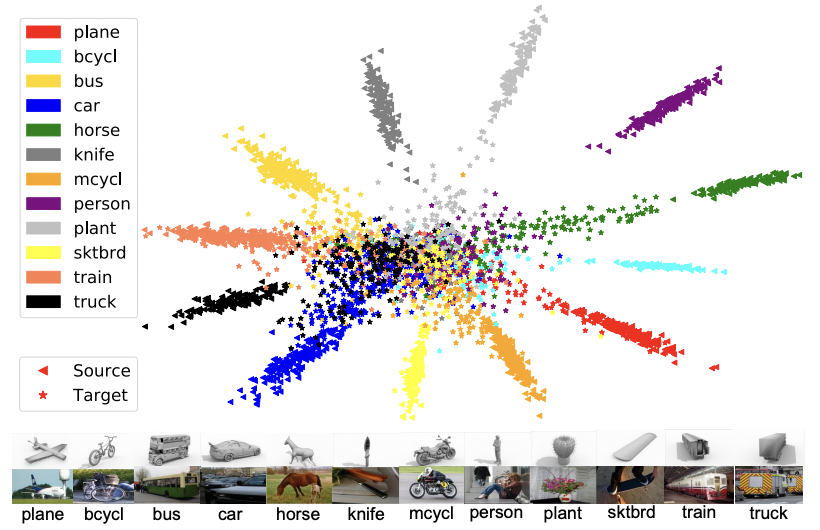
\includegraphics[width=0.7\textwidth]{chapter2/afn-visda-source-only.png}

  \caption[Representación de características aprendidas de una CNN]{Visualización de las características aprendidas para el origen y destino utilizando un modelo entrenado utilizando muestras del origen. Imagen tomada de \cite{xu2019larger}.}
  \label{fig:afn-source-only}
\end{figure}

Esto sugiere que las normas excesivamente pequeñas de las muestras de destino con respecto a las de origen explican el
deterioro en la clasificación. No obstante, pueden plantearse dos hipótesis:

\begin{itemize}
  \item Normas de las características desalineadas: el desplazamiento entre los dominios de origen y destino se explica en la
        desalineación de los valores esperados de las normas de sus características. La coincidencia de las normas de ambos
        dominios a un escalar arbitrariamente elegido supondrá una mejora en la transferencias.
  \item Norma de las caracteristicas más pequeña: el desplazamiento entre los dominios se explica debido a las características
        menos informativas con normas más pequeñas del dominio de destino. Adaptar las características de destino a regiones
        alejadas de las normas pequeñas supondrá una mejora en la transferencia.
\end{itemize}

\cite{xu2019larger} propone un método llamado {\it Adaptive Feature Norm AFN} que consiste en normalizar las normas de las características aprendidas por la red $\mathcal{G}$  mediante $n$ bloques $\mathcal{N}$ (compuestos por FC-BN-ReLU-Dropout) y mediante $\mathcal{L}_{AFN}$.

\begin{figure}[H]
  \centering

  \tikzset{every picture/.style={line width=0.75pt}} %set default line width to 0.75pt        

  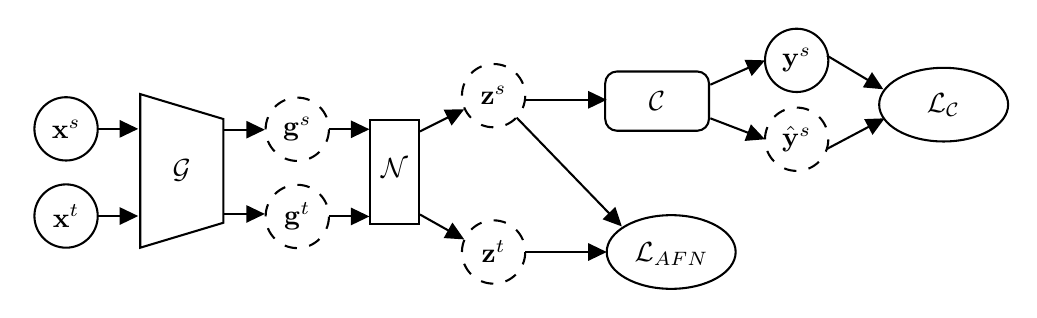
\begin{tikzpicture}[x=0.75pt,y=0.75pt,yscale=-1,xscale=1]
    %uncomment if require: \path (0,409); %set diagram left start at 0, and has height of 409

    %Shape: Circle [id:dp36883064074545446] 
    \draw   (59,84.75) .. controls (59,76.33) and (65.83,69.5) .. (74.25,69.5) .. controls (82.67,69.5) and (89.5,76.33) .. (89.5,84.75) .. controls (89.5,93.17) and (82.67,100) .. (74.25,100) .. controls (65.83,100) and (59,93.17) .. (59,84.75) -- cycle ;

    %Shape: Circle [id:dp7170555789489086] 
    \draw   (59,126.75) .. controls (59,118.33) and (65.83,111.5) .. (74.25,111.5) .. controls (82.67,111.5) and (89.5,118.33) .. (89.5,126.75) .. controls (89.5,135.17) and (82.67,142) .. (74.25,142) .. controls (65.83,142) and (59,135.17) .. (59,126.75) -- cycle ;

    %Shape: Trapezoid [id:dp6591706550778527] 
    \draw   (110,68) -- (150,80) -- (150,130) -- (110,142) -- cycle ;

    %Straight Lines [id:da8866180371172607] 
    \draw    (89.5,84.75) -- (106,84.75) ;
    \draw [shift={(109,84.75)}, rotate = 180] [fill={rgb, 255:red, 0; green, 0; blue, 0 }  ][line width=0.08]  [draw opacity=0] (8.93,-4.29) -- (0,0) -- (8.93,4.29) -- cycle    ;
    %Shape: Circle [id:dp7226735192986846] 
    \draw  [dash pattern={on 4.5pt off 4.5pt}] (264.98,68.75) .. controls (264.98,60.33) and (271.81,53.5) .. (280.23,53.5) .. controls (288.66,53.5) and (295.48,60.33) .. (295.48,68.75) .. controls (295.48,77.17) and (288.66,84) .. (280.23,84) .. controls (271.81,84) and (264.98,77.17) .. (264.98,68.75) -- cycle ;
    %Shape: Circle [id:dp11338914726883309] 
    \draw  [dash pattern={on 4.5pt off 4.5pt}] (264.98,144.08) .. controls (264.98,135.66) and (271.81,128.83) .. (280.23,128.83) .. controls (288.66,128.83) and (295.48,135.66) .. (295.48,144.08) .. controls (295.48,152.51) and (288.66,159.33) .. (280.23,159.33) .. controls (271.81,159.33) and (264.98,152.51) .. (264.98,144.08) -- cycle ;
    %Straight Lines [id:da7817124779055846] 
    \draw    (89.5,126.75) -- (106,126.75) ;
    \draw [shift={(109,126.75)}, rotate = 180] [fill={rgb, 255:red, 0; green, 0; blue, 0 }  ][line width=0.08]  [draw opacity=0] (8.93,-4.29) -- (0,0) -- (8.93,4.29) -- cycle    ;
    %Straight Lines [id:da7526972599979318] 
    \draw    (244.73,86) -- (263.38,76.67) ;
    \draw [shift={(266.07,75.33)}, rotate = 153.43] [fill={rgb, 255:red, 0; green, 0; blue, 0 }  ][line width=0.08]  [draw opacity=0] (8.93,-4.29) -- (0,0) -- (8.93,4.29) -- cycle    ;
    %Straight Lines [id:da13505401193908728] 
    \draw    (244.73,126) -- (263.45,136.53) ;
    \draw [shift={(266.07,138)}, rotate = 209.36] [fill={rgb, 255:red, 0; green, 0; blue, 0 }  ][line width=0.08]  [draw opacity=0] (8.93,-4.29) -- (0,0) -- (8.93,4.29) -- cycle    ;
    %Straight Lines [id:da4909359959704669] 
    \draw    (295.48,70.75) -- (331.73,70.75) ;
    \draw [shift={(334.73,70.75)}, rotate = 180] [fill={rgb, 255:red, 0; green, 0; blue, 0 }  ][line width=0.08]  [draw opacity=0] (8.93,-4.29) -- (0,0) -- (8.93,4.29) -- cycle    ;
    %Straight Lines [id:da25373400738229757] 
    \draw    (295.48,144.08) -- (331.73,144.08) ;
    \draw [shift={(334.73,144.08)}, rotate = 180] [fill={rgb, 255:red, 0; green, 0; blue, 0 }  ][line width=0.08]  [draw opacity=0] (8.93,-4.29) -- (0,0) -- (8.93,4.29) -- cycle    ;
    %Shape: Rectangle [id:dp03201668448552586] 
    \draw   (220.67,80.6) -- (244.33,80.6) -- (244.33,130.4) -- (220.67,130.4) -- cycle ;

    %Shape: Circle [id:dp0590517882755186] 
    \draw  [dash pattern={on 4.5pt off 4.5pt}] (170.4,84.95) .. controls (170.4,76.53) and (177.23,69.7) .. (185.65,69.7) .. controls (194.07,69.7) and (200.9,76.53) .. (200.9,84.95) .. controls (200.9,93.37) and (194.07,100.2) .. (185.65,100.2) .. controls (177.23,100.2) and (170.4,93.37) .. (170.4,84.95) -- cycle ;
    %Shape: Circle [id:dp9792876246953977] 
    \draw  [dash pattern={on 4.5pt off 4.5pt}] (170.4,126.95) .. controls (170.4,118.53) and (177.23,111.7) .. (185.65,111.7) .. controls (194.07,111.7) and (200.9,118.53) .. (200.9,126.95) .. controls (200.9,135.37) and (194.07,142.2) .. (185.65,142.2) .. controls (177.23,142.2) and (170.4,135.37) .. (170.4,126.95) -- cycle ;
    %Straight Lines [id:da9352682997505948] 
    \draw    (200.9,84.95) -- (217.4,84.95) ;
    \draw [shift={(220.4,84.95)}, rotate = 180] [fill={rgb, 255:red, 0; green, 0; blue, 0 }  ][line width=0.08]  [draw opacity=0] (8.93,-4.29) -- (0,0) -- (8.93,4.29) -- cycle    ;
    %Straight Lines [id:da9288909607910223] 
    \draw    (200.9,126.95) -- (217.4,126.95) ;
    \draw [shift={(220.4,126.95)}, rotate = 180] [fill={rgb, 255:red, 0; green, 0; blue, 0 }  ][line width=0.08]  [draw opacity=0] (8.93,-4.29) -- (0,0) -- (8.93,4.29) -- cycle    ;
    %Straight Lines [id:da42477525756570467] 
    \draw    (150.5,85.15) -- (167,85.15) ;
    \draw [shift={(170,85.15)}, rotate = 180] [fill={rgb, 255:red, 0; green, 0; blue, 0 }  ][line width=0.08]  [draw opacity=0] (8.93,-4.29) -- (0,0) -- (8.93,4.29) -- cycle    ;
    %Straight Lines [id:da19510792007996902] 
    \draw    (150.5,125.75) -- (167,125.75) ;
    \draw [shift={(170,125.75)}, rotate = 180] [fill={rgb, 255:red, 0; green, 0; blue, 0 }  ][line width=0.08]  [draw opacity=0] (8.93,-4.29) -- (0,0) -- (8.93,4.29) -- cycle    ;
    %Rounded Rect [id:dp8233373593250533] 
    \draw   (334,62.81) .. controls (334,59.65) and (336.56,57.1) .. (339.71,57.1) -- (378.29,57.1) .. controls (381.44,57.1) and (384,59.65) .. (384,62.81) -- (384,79.95) .. controls (384,83.11) and (381.44,85.67) .. (378.29,85.67) -- (339.71,85.67) .. controls (336.56,85.67) and (334,83.11) .. (334,79.95) -- cycle ;

    %Shape: Circle [id:dp361141070335256] 
    \draw   (411,51.75) .. controls (411,43.33) and (417.83,36.5) .. (426.25,36.5) .. controls (434.67,36.5) and (441.5,43.33) .. (441.5,51.75) .. controls (441.5,60.17) and (434.67,67) .. (426.25,67) .. controls (417.83,67) and (411,60.17) .. (411,51.75) -- cycle ;
    %Shape: Circle [id:dp994981759860698] 
    \draw  [dash pattern={on 4.5pt off 4.5pt}] (411,89.75) .. controls (411,81.33) and (417.83,74.5) .. (426.25,74.5) .. controls (434.67,74.5) and (441.5,81.33) .. (441.5,89.75) .. controls (441.5,98.17) and (434.67,105) .. (426.25,105) .. controls (417.83,105) and (411,98.17) .. (411,89.75) -- cycle ;
    %Shape: Ellipse [id:dp4863694749188221] 
    \draw   (466,73.08) .. controls (466,63.28) and (479.91,55.33) .. (497.06,55.33) .. controls (514.22,55.33) and (528.13,63.28) .. (528.13,73.08) .. controls (528.13,82.89) and (514.22,90.83) .. (497.06,90.83) .. controls (479.91,90.83) and (466,82.89) .. (466,73.08) -- cycle ;
    %Straight Lines [id:da7034112467211542] 
    \draw    (384.67,63.48) -- (408.26,52.97) ;
    \draw [shift={(411,51.75)}, rotate = 156] [fill={rgb, 255:red, 0; green, 0; blue, 0 }  ][line width=0.08]  [draw opacity=0] (8.93,-4.29) -- (0,0) -- (8.93,4.29) -- cycle    ;
    %Straight Lines [id:da28235679904283506] 
    \draw    (384.67,79.67) -- (408.2,88.68) ;
    \draw [shift={(411,89.75)}, rotate = 200.95] [fill={rgb, 255:red, 0; green, 0; blue, 0 }  ][line width=0.08]  [draw opacity=0] (8.93,-4.29) -- (0,0) -- (8.93,4.29) -- cycle    ;
    %Straight Lines [id:da3443605473479898] 
    \draw    (440.83,49.42) -- (465.43,64.13) ;
    \draw [shift={(468,65.67)}, rotate = 210.89] [fill={rgb, 255:red, 0; green, 0; blue, 0 }  ][line width=0.08]  [draw opacity=0] (8.93,-4.29) -- (0,0) -- (8.93,4.29) -- cycle    ;
    %Straight Lines [id:da6547044180228383] 
    \draw    (440.83,94.42) -- (466.02,81.07) ;
    \draw [shift={(468.67,79.67)}, rotate = 152.08] [fill={rgb, 255:red, 0; green, 0; blue, 0 }  ][line width=0.08]  [draw opacity=0] (8.93,-4.29) -- (0,0) -- (8.93,4.29) -- cycle    ;
    %Straight Lines [id:da7710823975987622] 
    \draw    (291.33,79.33) -- (339.91,129.59) ;
    \draw [shift={(342,131.75)}, rotate = 225.97] [fill={rgb, 255:red, 0; green, 0; blue, 0 }  ][line width=0.08]  [draw opacity=0] (8.93,-4.29) -- (0,0) -- (8.93,4.29) -- cycle    ;
    %Shape: Ellipse [id:dp8075338571919093] 
    \draw   (334.73,144.08) .. controls (334.73,134.28) and (348.64,126.33) .. (365.8,126.33) .. controls (382.95,126.33) and (396.86,134.28) .. (396.86,144.08) .. controls (396.86,153.89) and (382.95,161.83) .. (365.8,161.83) .. controls (348.64,161.83) and (334.73,153.89) .. (334.73,144.08) -- cycle ;

    % Text Node
    \draw (130,105) node   [align=left] {\begin{minipage}[lt]{22.78pt}\setlength\topsep{0pt}
        \begin{center}
          $\mathcal{G}$
        \end{center}

      \end{minipage}};
    % Text Node
    \draw (74.25,126.75) node   [align=left] {\begin{minipage}[lt]{21.08pt}\setlength\topsep{0pt}
        \begin{center}
          $\mathbf{x}^t$
        \end{center}

      \end{minipage}};
    % Text Node
    \draw (74.25,84.75) node   [align=left] {\begin{minipage}[lt]{21.08pt}\setlength\topsep{0pt}
        \begin{center}
          $\mathbf{x}^s$
        \end{center}

      \end{minipage}};
    % Text Node
    \draw (221,97.4) node [anchor=north west][inner sep=0.75pt]   [align=left] {\begin{minipage}[lt]{15pt}\setlength\topsep{0pt}
        \begin{center}
          $\mathcal{N}$
        \end{center}

      \end{minipage}};
    % Text Node
    \draw (185.65,84.95) node   [align=left] {\begin{minipage}[lt]{21.08pt}\setlength\topsep{0pt}
        \begin{center}
          $\mathbf{g}^s$
        \end{center}

      \end{minipage}};
    % Text Node
    \draw (185.65,126.95) node   [align=left] {\begin{minipage}[lt]{21.08pt}\setlength\topsep{0pt}
        \begin{center}
          $\mathbf{g}^t$
        \end{center}

      \end{minipage}};
    % Text Node
    \draw (426.25,51.75) node   [align=left] {\begin{minipage}[lt]{21.08pt}\setlength\topsep{0pt}
        \begin{center}
          $\mathbf{y}^s$
        \end{center}

      \end{minipage}};
    % Text Node
    \draw (426.25,89.75) node   [align=left] {\begin{minipage}[lt]{21.08pt}\setlength\topsep{0pt}
        \begin{center}
          $\hat{\mathbf{y}}^s$
        \end{center}

      \end{minipage}};
    % Text Node
    \draw (497.06,73.08) node   [align=left] {\begin{minipage}[lt]{32.64pt}\setlength\topsep{0pt}
        \begin{center}
          $\mathcal{L}_{\mathcal{C}}$
        \end{center}

      \end{minipage}};
    % Text Node
    \draw (359,71.56) node   [align=left] {\begin{minipage}[lt]{26.23pt}\setlength\topsep{0pt}
        \begin{center}
          $\mathcal{C}$
        \end{center}

      \end{minipage}};
    % Text Node
    \draw (366,145) node   [align=left] {\begin{minipage}[lt]{35pt}\setlength\topsep{0pt}
        \begin{center}
          $\mathcal{L}_{AFN}$
        \end{center}

      \end{minipage}};
    % Text Node
    \draw (280.23,144.08) node   [align=left] {\begin{minipage}[lt]{21.08pt}\setlength\topsep{0pt}
        \begin{center}
          $\mathbf{z}^t$
        \end{center}

      \end{minipage}};
    % Text Node
    \draw (280.23,68.75) node   [align=left] {\begin{minipage}[lt]{21.08pt}\setlength\topsep{0pt}
        \begin{center}
          $\mathbf{z}^s$
        \end{center}

      \end{minipage}};

  \end{tikzpicture}
  \caption[Esquema de {\it AFN}]{Esquema de {\it AFN}. Los supra indices $s$ y $t$ indican si los datos son del origen o destino respectivamente.
  Los círculos con líneas rayadas son salidas de los modelos mientras que los círculos de líneas sólidas son datos conocidos. El modelo {\it backbone} $\mathcal{G}$ produce características $\mathbf{x}$ que luego son aplicadas por bloques $\mathcal{N}$ (FC-BN-ReLU-Dropout) produciendo características normalizadas $\mathbf{d}$. La red clasificadora $\mathcal{C}$ toma las características $\mathbf{d}^s$ y se computa $\mathcal{L}_{\mathcal{C}}$. $\mathcal{L}_{AFN}$ se calcula utilizando $\mathbf{d}$.}
  \label{fig:afn-esquema}
\end{figure}

En su variante iterativa, $\mathcal{L}_{AFN}$ se define como:

\begin{align}
  \min_{\mathcal{G}} \mathcal{L}_{AFN}(\mathbf{x}^s, \mathbf{x}^t) = & \mathbb{E}_{\mathbf{x}^s \sim \mathcal{\hat{S}}} \mathbb{E}[(\| \mathcal{G}(\mathcal{N}(\mathbf{x}^s)) \| - \Delta_r)^2] \nonumber \\
                                                                     & + \mathbb{E}_{\mathbf{x}^t \sim \mathcal{\hat{T}}} \mathbb{E}[(\| \mathcal{G}(\mathcal{N}(\mathbf{x}^t)) \| - \Delta_r)^2]
  \label{eq:afn-loss}
\end{align}

Donde $\Delta_r$ corresponde al escalar que controla la amplitud de la norma. Los autores afirman que puede agregarse
un término a la ecuación \ref{eq:afn-loss} respecto a la entropía $\mathcal{H}$ de la función {\it softmax} $\sigma$
para facilitar la discriminabilidad mediante un factor $\beta$:

\begin{align}
  \min_{\mathcal{G}} \mathcal{L}_{AFN}(\mathbf{x}^s, \mathbf{x}^t) = & \mathbb{E}_{\mathbf{x}^s \sim \mathcal{\hat{S}}} \mathbb{E}[(\| \mathcal{G}(\mathcal{N}(\mathbf{x}^s)) \| - \Delta_r)^2] \nonumber   \\
                                                                     & + \mathbb{E}_{\mathbf{x}^t \sim \mathcal{\hat{T}}} \mathbb{E}[(\| \mathcal{G}(\mathcal{N}(\mathbf{x}^t)) \| - \Delta_r)^2] \nonumber \\
                                                                     & + \beta \mathcal{H}(\sigma(\mathcal{G}(\mathcal{N}(\mathbf{x}^s)) ))
  \label{eq:afn-loss-entropy}
\end{align}

Por lo tanto, el objetivo de optimización viene dado por la ecuación \ref{eq:afn-objetivo}, donde $\lambda$ es el
trade-off entre la clasificación y normalizacion de normas.

\begin{align}
  \min_{\mathcal{G}, \mathcal{C}} \mathcal{L}_{\mathcal{C}}(\mathbf{x}^s, \mathbf{x}^t) + \lambda \mathcal{L}_{\mathcal{AFN}}(\mathbf{x}^s, \mathbf{x}^t)
  \label{eq:afn-objetivo}
\end{align}